\documentclass[a4paper,12pt,twoside]{memoir}

% Castellano
\usepackage[spanish,es-tabla]{babel}
\selectlanguage{spanish}
\usepackage[utf8]{inputenc}
\usepackage[T1]{fontenc}
\usepackage{lmodern} % scalable font
\usepackage{microtype}
\usepackage{placeins}
\usepackage[numbers]{natbib}
\usepackage{url}
\usepackage{float}
\usepackage{listings}


%Para insertar código
\lstset{
    language=C++,                % Lenguaje del código
    basicstyle=\ttfamily\footnotesize, % Estilo de la fuente
    keywordstyle=\color{blue},        % Estilo de palabras clave
    stringstyle=\color{green},        % Estilo de cadenas
    commentstyle=\color{gray},        % Estilo de comentarios
    morecomment=[l][\color{magenta}]{\#}, % Estilo de comentarios con #
    numbers=left,                    % Numeración de líneas a la izquierda
    numberstyle=\tiny\color{gray},   % Estilo de los números de línea
    stepnumber=1,                    % Mostrar cada línea
    numbersep=5pt,                   % Separación de los números de línea
    backgroundcolor=\color{white},   % Color de fondo
    showspaces=false,                % No mostrar espacios
    showstringspaces=false,          % No mostrar espacios en las cadenas
    breaklines=true,                 % Dividir líneas largas
    breakatwhitespace=true,          % Dividir líneas en espacios
    tabsize=2,                       % Tamaño del tabulador
    columns=fullflexible,
    keepspaces=true
}

\RequirePackage{booktabs}
\RequirePackage[table]{xcolor}
\RequirePackage{xtab}
\RequirePackage{multirow}

% Links
\PassOptionsToPackage{hyphens}{url}\usepackage[colorlinks]{hyperref}
\hypersetup{
	allcolors = {red}
}

% Ecuaciones
\usepackage{amsmath}

% Rutas de fichero / paquete
\newcommand{\ruta}[1]{{\sffamily #1}}

% Párrafos
\nonzeroparskip

% Huérfanas y viudas
\widowpenalty100000
\clubpenalty100000

% Evitar solapes en el header
\nouppercaseheads


\let\tmp\oddsidemargin
\let\oddsidemargin\evensidemargin
\let\evensidemargin\tmp
\reversemarginpar



% Imagenes
\usepackage{graphicx}
\newcommand{\imagen}[2]{
	\begin{figure}[!h]
		\centering
		\includegraphics[width=0.9\textwidth]{#1}
		\caption{#2}\label{fig:#1}
	\end{figure}
	\FloatBarrier
}






\graphicspath{ {./img/} }

% Capítulos
\chapterstyle{bianchi}
\newcommand{\capitulo}[2]{
	\setcounter{chapter}{#1}
	\setcounter{section}{0}
	\setcounter{figure}{0}
	\setcounter{table}{0}
	\chapter*{#2}
	\addcontentsline{toc}{chapter}{#2}
	\markboth{#2}{#2}
}

% Apéndices
\renewcommand{\appendixname}{Apéndice}
\renewcommand*\cftappendixname{\appendixname}

\newcommand{\apendice}[1]{
	%\renewcommand{\thechapter}{A}
	\chapter{#1}
}

\renewcommand*\cftappendixname{\appendixname\ }

% Formato de portada
\makeatletter
\usepackage{xcolor}
\newcommand{\tutor}[1]{\def\@tutor{#1}}
\newcommand{\tutorb}[1]{\def\@tutorb{#1}}
\newcommand{\course}[1]{\def\@course{#1}}
\definecolor{cpardoBox}{HTML}{E6E6FF}
\def\maketitle{
  \null
  \thispagestyle{empty}
  % Cabecera ----------------
\begin{center}
  \noindent
\includegraphics[width=\textwidth]{cabeceraSalud}\vspace{1.5cm}%
\end{center}
  
  % Título proyecto y escudo salud ----------------
  \begin{center}
    \begin{minipage}[c][1.5cm][c]{.20\textwidth}
        
\includegraphics[width=\textwidth]{escudoSalud.pdf}
    \end{minipage}
  \end{center}
  
  \begin{center}
    \colorbox{cpardoBox}{%
        \begin{minipage}{.8\textwidth}
          \vspace{.5cm}\Large
          \begin{center}
          \textbf{TFG del Grado en Ingeniería de la Salud}\vspace{.6cm}\\
          \textbf{\LARGE\@title{}}
          \end{center}
          \vspace{.2cm}
        \end{minipage}
    }%
  \end{center}
  
    % Datos de alumno, curso y tutores ------------------
  \begin{center}%
  {%
    \noindent\LARGE
    Presentado por \@author{}\\ 
    en Universidad de Burgos\\
    \vspace{0.5cm}
    \noindent\Large
    \@date{}\\
    \vspace{0.5cm}
    Tutor: \@tutor{}\\ % comenta el que no corresponda
    %Tutores: \@tutor{} -- \@tutorb{}\\
  }%
  \end{center}%
  \null
  \cleardoublepage
  }
\makeatother



% Datos de portada
\title{Desarrollo de una derivación ventriculoperitoneal con sensor de presión intracraneal para tratar la hidrocefalia \\Documentación Técnica}
\author{Celia Valladolid Portal}
\tutor{Guirguis Zaki Guirguis Abdelmessih}
%\tutorb{nombre tutor 2}
\date{\today}

\begin{document}

\maketitle



\cleardoublepage



%%%%%%%%%%%%%%%%%%%%%%%%%%%%%%%%%%%%%%%%%%%%%%%%%%%%%%%%%%%%%%%%%%%%%%%%%%%%%%%%%%%%%%%%



\frontmatter


\clearpage

% Indices
\tableofcontents

\clearpage

\listoffigures

\clearpage

\listoftables

\clearpage

\mainmatter

\appendix




\apendice{Plan de Proyecto Software}

\section{Introducción}
En este primer anexo se ofrece la planificación temporal seguida a lo largo del proyecto, así como una planificación del coste que conlleva el prototipo realizado. Por último se analizará la viabilidad legal contemplando las leyes pertinentes para el desarrollo de este proyecto.


\section{Planificación temporal}

En este apartado se va a recoger la información relativa a la planificación temporal del proyecto. Se ha empleado GitHub para la organización del proyecto, a través de \textit{Issues} específicas. Para etiquetar las tareas se han usado diferentes \textit{labels} que describen en qué consiste cada tarea. Todo esto lo podemos ver en este \href{https://github.com/CeliaValladolid/TFG_Valvula_Derivacion_VentriculoPeritoneal}{Repositorio}.
A continuación, en la Figura \ref{fig:planificación} podemos observar la planificación seguida y distribuida por semanas.
\begin{figure}[h]
    \centering
    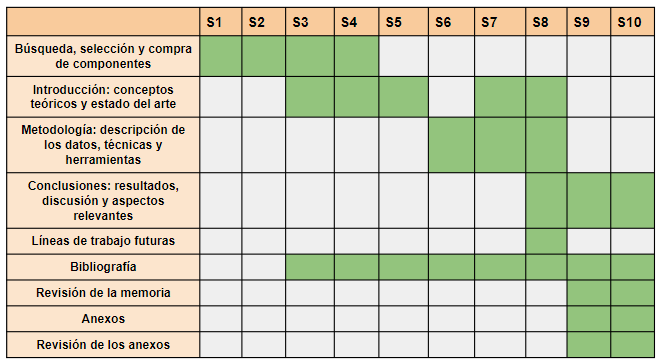
\includegraphics[width=1.1\textwidth]{img/planificacion.PNG}
    \caption{Planificación temporal. Imagen propia}
    \label{fig:planificación}
\end{figure}

\subsection{Planificación económica}

La evaluación del coste asociado a este proyecto se puede desglosar en tres partes, por un lado el gasto en hardware, por otro el gasto en software y por último el gasto personal, el gasto que conlleva sacar adelante este trabajo.

\subsubsection{Coste hardware}
Como elemento principal se necesita un ordenador, en mi caso es un Asus bastante antiguo pero si hoy en día tuviésemos que comprar uno, necesitaríamos aproximadamente unos 600€ tirando por lo bajo.

En cuanto a los componentes electrónicos:
\begin{itemize}
    \item Placa Arduino Uno R3 \cite{compraplaca}: 29,04€
    \item ProtoBoard \cite{compraproto}: 5,49€
    \item Cableado \cite{compracables}: 9,98€
    \item Cable USB \cite{comprausb}: 3,96€
    \item Sensor de presión NXP MPX5010DP \cite{comprasensor}: 22,01€ + 7,77€ (IVA) + 14,99€ (gastos de envío) = 44,77€
    \item Mini bomba \cite{comprabomba}: 7,59€ (2 ud)
    \item Relé \cite{comprarele}: 5,49€
    \item Portapilas \cite{compraporta}: 6,50€
    \item Pilas: 2€
\end{itemize}
En la siguiente tabla \ref{tab:costes} podemos ver la suma total de todo el hardware necesario.

\begin{table}[h!]
\centering
\begin{tabular}{ |c|c| }
\hline
\rowcolor[HTML]{B0E0E6} 
\textbf{Componente} & \textbf{Coste} \\
\hline
Ordenador ASUS & 600€ \\
\hline
Placa Arduino Uno R3 & 29,04€ \\
\hline
ProtoBoard & 5,49€ \\
\hline
Cableado & 9,98€ \\
\hline
Cable USB & 3,96€ \\
\hline
Sensor de presión NXP MPX5010DP & 44,77€ \\
\hline
Mini bomba & 3,79€ \\
\hline
Relé & 5,49€ \\
\hline
Portapilas & 6,50€ \\
\hline
Pilas & 2€ \\
\hline
Tubo para el sensor & 1€ \\
\hline
\rowcolor[HTML]{4682B4} 
\textbf{Total} & \textbf{712,02€} \\
\hline
\end{tabular}
\caption{Resumen de costes de hardware}
\label{tab:costes}
\end{table}

\subsubsection{Coste software}
Los costes del software empleado para elaborar el proyecto han sido nulos debido a que se han empleado aplicaciones, plataformas y entornos de código abierto en los que su uso es gratuito. 

\subsubsection{Coste de personal}
Respecto al coste de personal, vamos a suponer que el salario bruto\footnote{El salario bruto hace referencia a la cantidad de dinero que percibe el empleado antes de aplicarle las deducciones por IRPF y las cotizaciones a la Seguridad Social mientras que la cantidad total a percibir se denomina salario neto \cite{bruto}. } de un ingeniero de la salud con poca experiencia no supera los 20.000€ anuales, por lo tanto aplicando las deducciones pertinentes obtenemos las cifras recogidas en las tablas \ref{tab:costes-personal} \ref{tab:costes-personal1}.

\begin{table}[h!]
\centering
\begin{tabular}{ |c|c| }
\hline
\rowcolor[HTML]{B0E0E6} 
\textbf{Concepto} & \textbf{Coste} \\
\hline
Salario bruto anual & 20.000€ \\
\hline
Retención IRPF anual & 1.772€ \\
\hline
Cuotas a la Seguridad Social (año) & 1.349,69€ \\
\hline
\rowcolor[HTML]{4682B4} 
\textbf{Sueldo neto anual} & \textbf{16.880,31€} \\
\hline
\end{tabular}
\caption{Resumen de costes anuales de personal}
\label{tab:costes-personal}
\end{table}


\begin{table}[h!]
\centering
\begin{tabular}{ |c|c| }
\hline
\rowcolor[HTML]{B0E0E6} 
\textbf{Concepto} & \textbf{Coste} \\
\hline
Salario bruto mensual & 1.666,66€ \\
\hline
Retención IRPF mensual & 147,66€ \\
\hline
Cuotas a la Seguridad Social (mes) & 112,47€ \\
\hline
Sueldo neto mensual & 1.406,53€ \\
\rowcolor[HTML]{4682B4} 
\textbf{Sueldo total 2 meses} & \textbf{2.813,06€} \\
\hline
\end{tabular}
\caption{Resumen de costes mensuales de personal}
\label{tab:costes-personal1}
\end{table}

\subsubsection{Coste total}
El coste total para desarrollar este proyecto, supone la suma de los gastos en hardware y en personal, recogidos en la tabla \ref{tab:costes-total}.

\begin{table}[h!]
\centering
\begin{tabular}{ |c|c| }
\hline
\rowcolor[HTML]{B0E0E6} 
\textbf{Concepto} & \textbf{Coste} \\
\hline
Hardware & 712,02€ \\
\hline
Personal & 2.813,06€ \\
\rowcolor[HTML]{4682B4} 
\textbf{Total} & \textbf{3.525,08€} \\
\hline
\end{tabular}
\caption{Resumen del coste total}
\label{tab:costes-total}
\end{table}

\subsection{Viabilidad legal}
En este apartado se abordan las leyes y normativas vigentes en la actualidad que hay que tener en cuenta para el desarrollo, comercialización y posterior tratamiento de los datos personales generados.

\subsubsection{Desarrollo y comercialización del dispositivo}
En este apartado se detallan las principales leyes, normativas y normas españolas y europeas encargadas de la regulación de los diferentes productos sanitarios y la protección de las invenciones en el campo de la tecnología médica.


La \textbf{Ley 24/2015}, más conocida como la Ley de Patentes \cite{patentes}, es la responsable de regular todo lo relacionado con la protección de invenciones a través de patentes, incluyendo aspectos como su registro, derecho a la patente y todos los procedimientos indispensables para poder solicitar una patente. Asimismo, el \textbf{Real Decreto Legislativo 1/1996}, relativo a la Ley de Propiedad Intelectual \cite{propintec}, es el encargado de regular la protección del derecho de autor y derechos semejantes.

En cuanto a los productos sanitarios, están regidos por la Agencia Española de Medicamentos y Productos Sanitarios (AEMPS). Destacan principalmente dos:
\begin{enumerate}
    \item \textbf{Real Decreto 437/2002} \cite{licencias}: regula todos los aspectos relacionados con los productos sanitarios, desde su desarrollo hasta su posterior comercialización.
    \item \textbf{Real Decreto 1591/2009} \cite{prod}: regula la concesión de las diferentes licencias necesarias para la fabricación y desarrollo del producto.
\end{enumerate}

En lo que respecta a los dispositivos que serán alojados en el interior del cuerpo humano, es fundamental el empleo de materiales biocompatibles. Este punto no afecta al prototipo desarrollado a lo largo del proyecto, pero sí que es un punto a tener en cuenta en el futuro, ya que la idea es desarrollar un dispositivo implantable en el interior del cráneo. Para ello, los materiales empleados deben ser compatibles con el tejido humano y no provocar ningún tipo de rechazo. Los dispositivos médicos implantables deben ser sometidos a rigurosos controles tales como pruebas de biocompatibilidad, estudios de toxicidad, y ensayos clínicos antes de su aprobación, con el objetivo de garantizar la eficacia y la seguridad del dispositivo y del paciente. 

La norma \textbf{ISO 10993-9:2022 - Evaluación Biológica de Productos Sanitarios} \cite{norma} es la encargada de regular la biocompatibilidad de los materiales utilizados para el desarrollo de los productos. Consta de una serie de normas internacionales que establecen distintos métodos para evaluar la seguridad de los materiales.


\subsubsection{Protección de datos personales}
En un proyecto que maneja datos sensibles de pacientes, es esencial incluir un apartado dedicado a la protección de estos datos para garantizar la privacidad de los individuos y el cumplimiento de las diferentes normativas legales vigentes. La protección de datos personales en el campo de la salud  está regulada por leyes y normativas tales como el \textbf{Reglamento General de Protección de Datos (RGPD)} o \textbf{Reglamento (UE) 2016/679} en la Unión Europea y la \textbf{Ley Orgánica 3/2018, de 5 de diciembre, de Protección de Datos Personales y garantía de los derechos digitales} en España. Estas leyes establecen principios fundamentales para el tratamiento de datos, como la licitud, exactitud, transparencia, integridad y confidencialidad así como la limitación tanto de la finalidad como del plazo de conservación y la minimización de datos .
\begin{itemize}
    \item El RGPD (Reglamento (UE) 2016/679) \cite{reglaue} establece los siguientes principios relativos al tratamiento de los datos recogidos:
    \begin{enumerate}
        \item \textbf{Tratados de manera lícita, leal y transparente} (Artículo 5.1.a): la recogida de los datos debe realizarse de forma justa y transparente, informando al individuo del posterior uso que recibirán sus datos.
        \item \textbf{Recogidos con fines determinados, explícitos y legítimos}(Artículo 5.1.b): los datos únicamente pueden ser empleados para los fines para los que fueron recogidos inicialmente.
        \item \textbf{Adecuados, pertinentes y limitados a lo necesario en relación con los fines para los que son tratados} (Artículo 5.1.c): solo se deben recoger los datos estrictamente necesarios para lograr el cumplimiento de los diferentes fines.
        \item \textbf{Exactos y, si fuera necesario, actualizados} (Artículo 5.1.d): se deben adoptar medidas razonables para garantizar que los datos inexactos con respecto a los fines se supriman o rectifiquen.
        \item \textbf{Mantenidos de forma que se permita la identificación de los interesados durante no más tiempo del necesario} (Artículo 5.1.e): los datos sólo deben ser conservados durante el tiempo necesario.
        \item \textbf{Tratados de tal manera que se garantice una seguridad adecuada de los datos personales} (Artículo 5.1.f): se deben implementar las medidas técnicas y organizativas pertinentes para proteger los datos contra su pérdida, destrucción, daño accidental o contra el tratamiento no autorizado o ilícito.
    \end{enumerate}
\end{itemize}
\begin{itemize}
    \item Por otra parte, la Ley Orgánica 3/2018, de 5 de diciembre, de Protección de Datos Personales y garantía de los derechos digitales \cite{leyorgdat} incluye algunos puntos adicionales, como:
    \begin{enumerate}
        \item \textbf{Tratamiento basado en el consentimiento del afectado} (Artículo 6): sólo será lícito el tratamiento de datos personales si el interesado  da su consentimiento inequívoco para una o varias finalidades. Por consentimiento se entiende toda manifestación de voluntad libre, específica, informada e inequívoca por la que este acepta el tratamiento de sus datos personales. Se debe asegurar que el afectado acepta y entiende las condiciones bajo las que sus datos serán tratados.
        \item \textbf{Derechos de los afectados} (Artículos 13-18): los individuos tienen derecho a acceder (13), rectificar (14), suprimir (15), limitar el tratamiento (16), solicitar la portabilidad (17) y oponerse (18) al tratamiento de los datos.
    \end{enumerate}
\end{itemize}

Uno de los aspectos más importantes cuando se trabaja con datos personales es la seguridad. La implementación de medidas de seguridad tales como el cifrado de contraseñas, la anonimización o el empleo de procedimientos seguros para llevar a cabo la transmisión de la información, resultan medidas indispensables para proteger los datos de una forma adecuada. Cabe destacar que el acceso al sistema debe estar restringido únicamente a personal autorizado.


Puede resultar realmente importante establecer un sistema que monitorice de forma ininterrumpida con el objetivo de detectar posibles violaciones de seguridad. En el caso de que esto ocurra, es fundamental tener un plan de respuesta que incluya la notificación del suceso a todos los afectados y a las autoridades pertinentes.


En resumen, la protección de datos personales es un punto clave cuando se elabora un proyecto que maneja información tan sensible como los datos de salud de los pacientes. Es una responsabilidad legal y ética, ya que proporciona confianza y fiabilidad al proyecto.


\apendice{Documentación de usuario}

\section{Requisitos software y hardware para ejecutar el proyecto}
En este apartado se van a tratar los requisitos de software y hardware necesarios para ejecutar el proyecto.

\subsection{Requisitos Software}
El único requisito de software para ejecutar el proyecto, es contar con la aplicación de Arduino IDE para poder compilar el código y poner en marcha el prototipo. Esta aplicación la podemos descargar \href{https://apps.microsoft.com/detail/9nblggh4rsd8?hl=es-es&gl=US}{aquí}.
Respecto a la aplicación para conseguir monitorizar al paciente, se establecen ciertos requisitos tales como:
\begin{enumerate}
    \item \textbf{Comunicación y transmisión instantánea de datos:} la importancia de que esta comunicación se realice de forma instantánea radica en la monitorización en tiempo real del paciente, pudiendo mandar notificaciones de alerta si se detectan lecturas fuera del rango establecido por el médico como "normal"\footnote{La presión intracraneal normal de una persona oscila entre los 5-15 mmHg}. Si está transmisión no es rápida, estos mensajes de alarma podrían llegar tarde, ocasionando complicaciones al paciente. Es importante que esta transmisión con el exterior se realice de forma inalámbrica, liberando de cables al paciente y velando por su comodidad. Un factor a tener en cuenta son las interferencias electromagnéticas presentes, por ejemplo, durante la realización de una resonancia magnética nuclear (RMN), por lo tanto es necesario que las técnicas y materiales empleados sean inertes a estas interferencias para evitar la distorsión de los resultados.
    \item \textbf{Accesibilidad:} la aplicación debe de ser accesible para el mayor número de personas posible a través de la identificación individual de cada usuario.
    \item \textbf{Interfaz intuitiva:} la interfaz de usuario debe ser intuitiva, fácil de usar y adaptada a las necesidades de los pacientes y requerimientos de los médicos.
    \item \textbf{Compatibilidad:} que sea compatible con diferentes sistemas operativos tales como Windows, Android, MacOS, IOS...
    \item \textbf{Seguridad y protección de datos:} al tratarse de datos de personas relacionados con la salud, se clasifican como datos muy sensibles por lo que deben de estar correctamente protegidos mediante la regulación de las leyes pertinentes. Esto lo podemos contemplar en el \textit{Anexo A, Viabilidad legal}. Se cuenta también con una serie de medidas que aseguren solo la entrada a la aplicación a usuarios autorizados.
    
\end{enumerate}


\subsection{Requisitos Hardware}
Los requisitos de hardware para desarrollar este trabajo es contar con los componentes recogidos en la tabla \ref{tab:costes}. Además, para mejorar este prototipo y conseguir un dispositivo funcional en personas, se debe tener en cuenta que cumpla con las siguientes características:
\begin{enumerate}
    \item \textbf{Tamaño, encapsulado y peso:} hacer hincapié en la miniaturización del dispositivo, conseguir que sea lo más pequeño posible para no ocasionar molestias al usuario. El encapsulado deberá de ser hermético para evitar la entrada de cualquier fluido, y biocompatible, ya que estará en contacto con tejido cerebral.
    \item \textbf{Durabilidad y resistencia:} deberá de ser resistente a la corrosión y tener una vida útil prolongada para evitar ser reemplazado a corto plazo. Es un requisito fundamental que el dispositivo sea duradero y resistente a posibles golpes.
    \item \textbf{Precisión y fiabilidad:} los sensores encargados de realizar las mediciones de los cambios de presión deberán ser de alta precisión y fiabilidad, realizando lecturas correctas y precisas sin margen de error.
    \item \textbf{Protección y seguridad:} todos los componentes del dispositivo deberán estar correctamente aislados, previniendo así cortocircuitos y daños en el paciente. 
    \item \textbf{Coste:} conseguir desarrollar un dispositivo de bajo coste sería ideal ya que lo haría accesible a más personas pero siempre debe primar la calidad del producto, haciéndolo de una forma segura y con los mejores materiales del mercado.
\end{enumerate}


\section{Instalación / Puesta en marcha}
Para la puesta en marcha necesitamos tener instalado la aplicación de Arduino en nuestro ordenador para poder compilar el código de una forma satisfactoria. En segundo lugar, debemos proceder al montaje del prototipo, contando con todos los componentes necesarios especificados en el \textit{Anexo A}. En la Figura \ref{fig:circuito} podemos ver el montaje completo del circuito.

\begin{figure}[h]
    \centering
    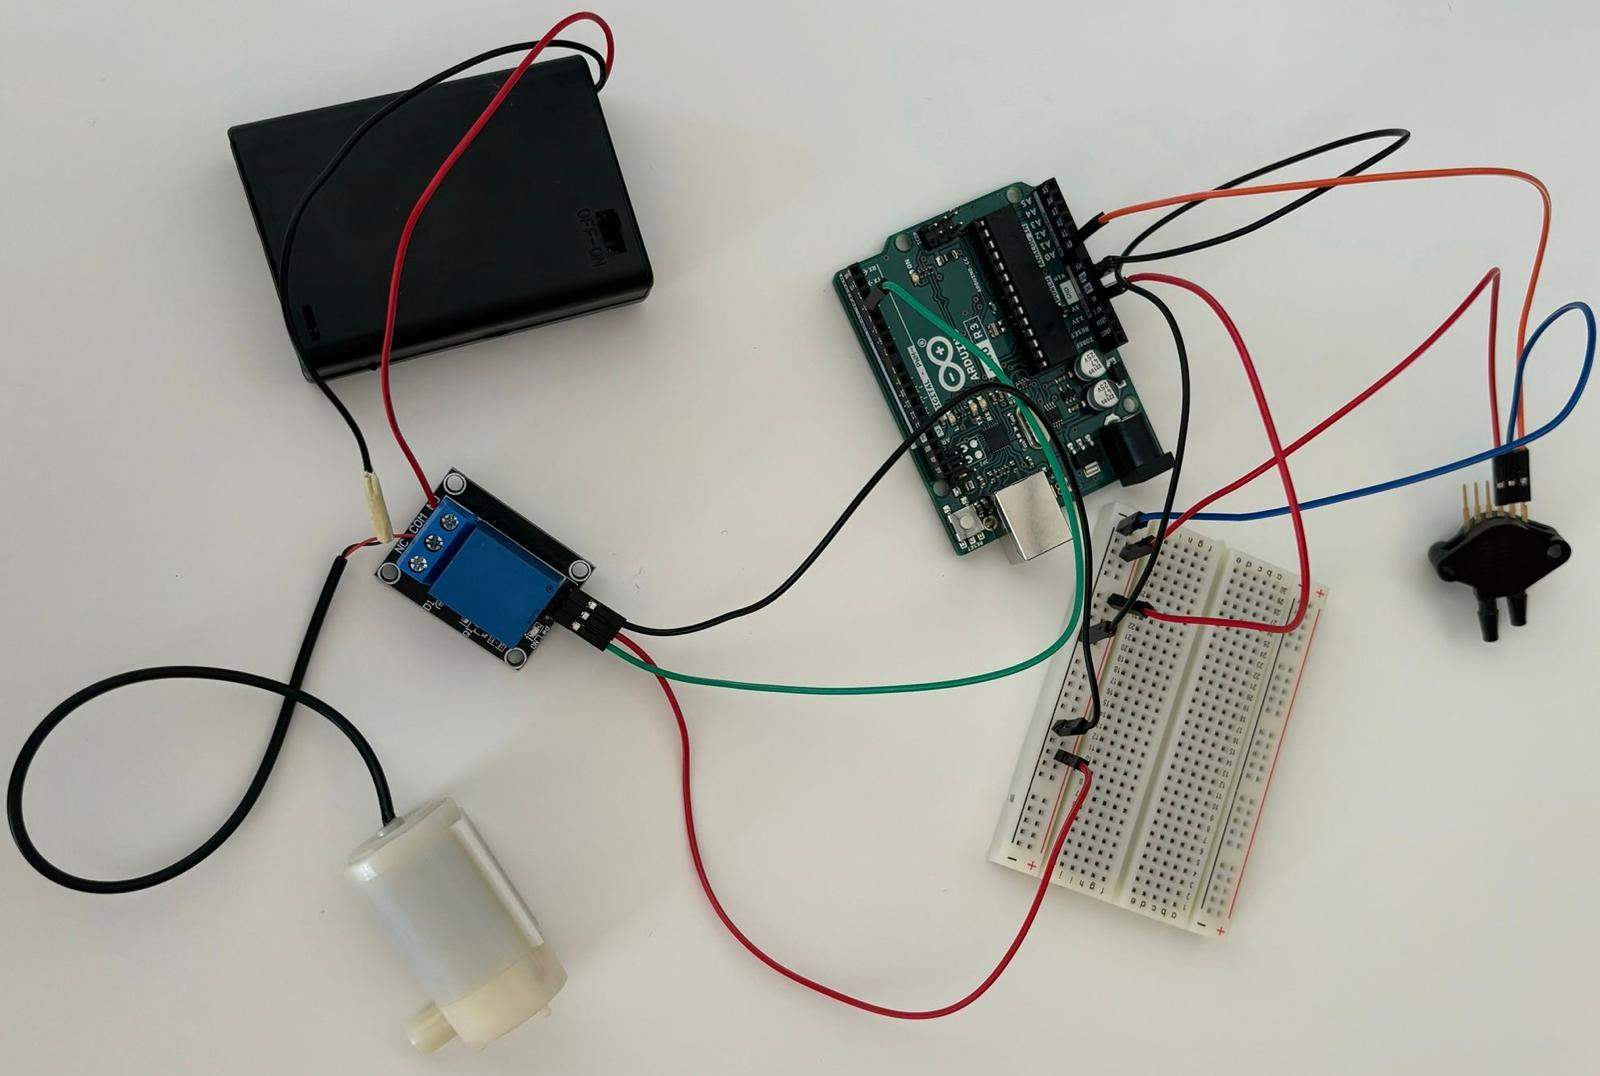
\includegraphics[width=0.9\textwidth]{img/circuitocompleto.jpg}
    \caption{Circuito electrónico. Imagen propia}
    \label{fig:circuito}
\end{figure}

El sensor se ha conectado de la siguiente manera. Su pinado consta de 6 pines, el pin 1 es el que presenta una muesca en la parte superior y va conectado a un pin analógico, A0 por ejemplo (cable azul). El pin 2 va conectado a GND (cable negro) y el pin 3 a 5V (cable rojo). Estas conexiones las podemos observar detalladamente en la Figura \ref{fig:conex_sens}.
\begin{figure}[h]
    \centering
    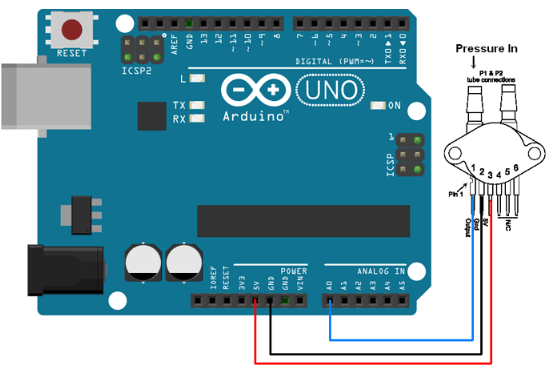
\includegraphics[width=0.9\textwidth]{img/conexion_sensr.PNG}
    \caption{Conexión sensor NPX MPX5010DP \cite{conexsen}}
    \label{fig:conex_sens}
\end{figure}

El relé, la mini bomba y la batería se han conectado entre ellas a la placa de Arduino. El relé es el encargado de hacer de interruptor, encendiendo y apagando la mini bomba, y la batería es necesaria para el suministro de corriente. El relé cuenta con tres pines y tres contactos. Los pines van conectados a la placa. El pin con el cable verde, va conectado a un pin digital, el del medio, cable rojo, a 5V y el siguiente, cable negro, a GND. Tanto la mini bomba como la batería cuentan con un cable rojo (+) y otro negro (-) cada una. El cable rojo de la mini bomba se introduce en el contacto común (C) del relé. Para ello es necesario utilizar un destornillador para aflojar un poco el tornillo y una vez introducido el cable lo apretamos para que se quede fijo y no se salga. Es importante que el cable que quede fuera del relé esté completamente aislado para que no ocurran cortocircuitos. El contacto común es el que se moverá abriendo o cerrando el circuito cuando se aplique corriente a la bobina y se genere el campo electromagnético, por eso el cable que debe ir ahí conectado es el del dispositivo que queremos controlar, en este caso, la mini bomba. El cable rojo de la batería irá al contacto normalmente abierto (NO) o al normalmente cerrado (NC), indistintamente. Por último se empalmarán los cables negros de la mini bomba y la batería, y quedarán juntos y correctacmente aislados. Para realizar el empalme sirve con quitar un poco del aislante que les recubre y entrelazar los filamentos entre ellos para que se produzca el contacto. En la Figura \ref{fig:conex_rele} podemos observar la conexión de estos tres componentes junto con la placa de Arduino.
\begin{figure}[h]
    \centering
    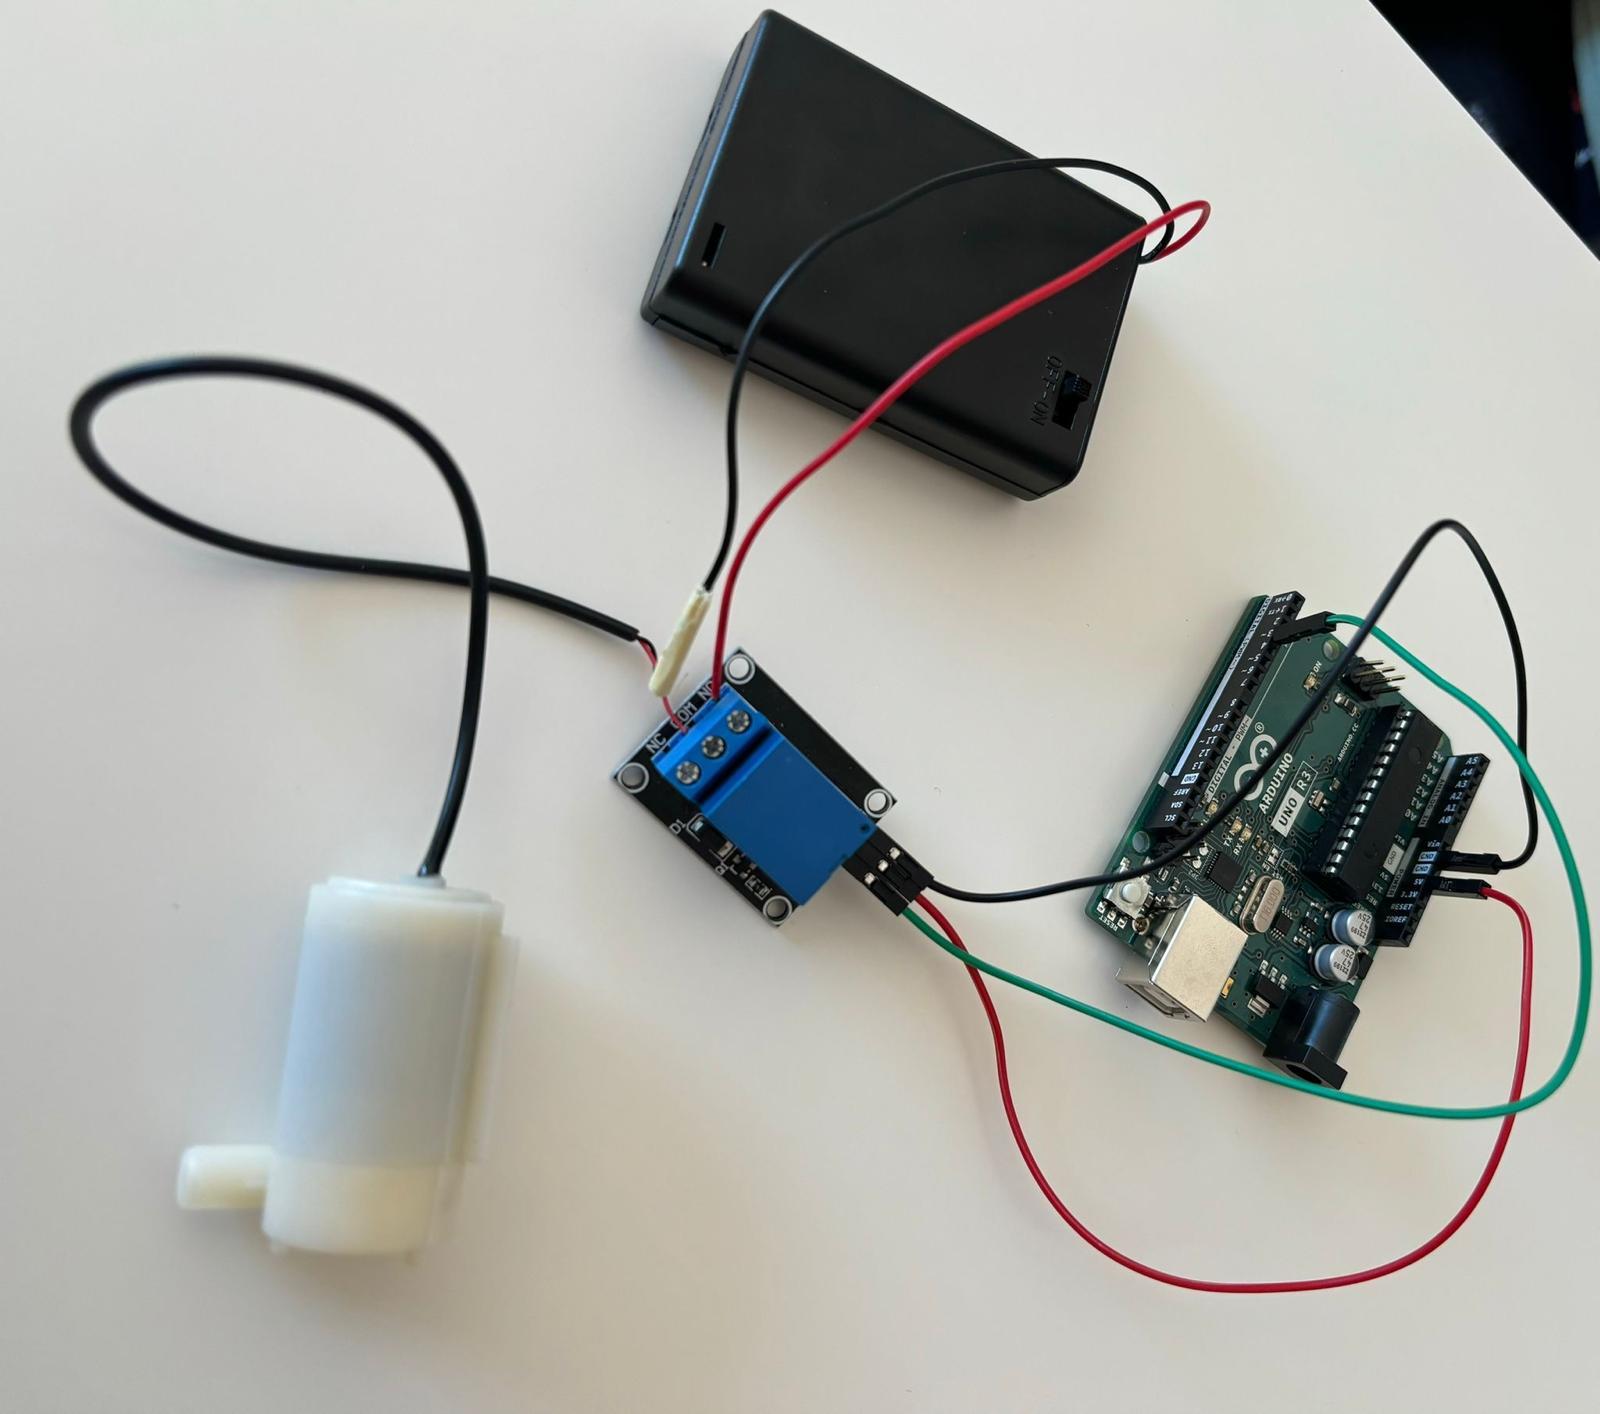
\includegraphics[width=0.9\textwidth]{img/rele-bomba.jpg}
    \caption{Conexión del relé, mini bomba y batería. Imagen propia}
    \label{fig:conex_rele}
\end{figure}

Con todo el circuito eléctrico montado, el último paso antes de conectarlo al ordenador, es colocar la manguera en la mini bomba y crear un colchón de aire al sensor (debido a que no se puede mojar) a través del empleo de otra manguera, tubo de plástico transparente, que irá introducido dentro del agua. El montaje del circuito completo lo podemos observar en la Figura \ref{fig:completo}.
\begin{figure}[H]
    \centering
    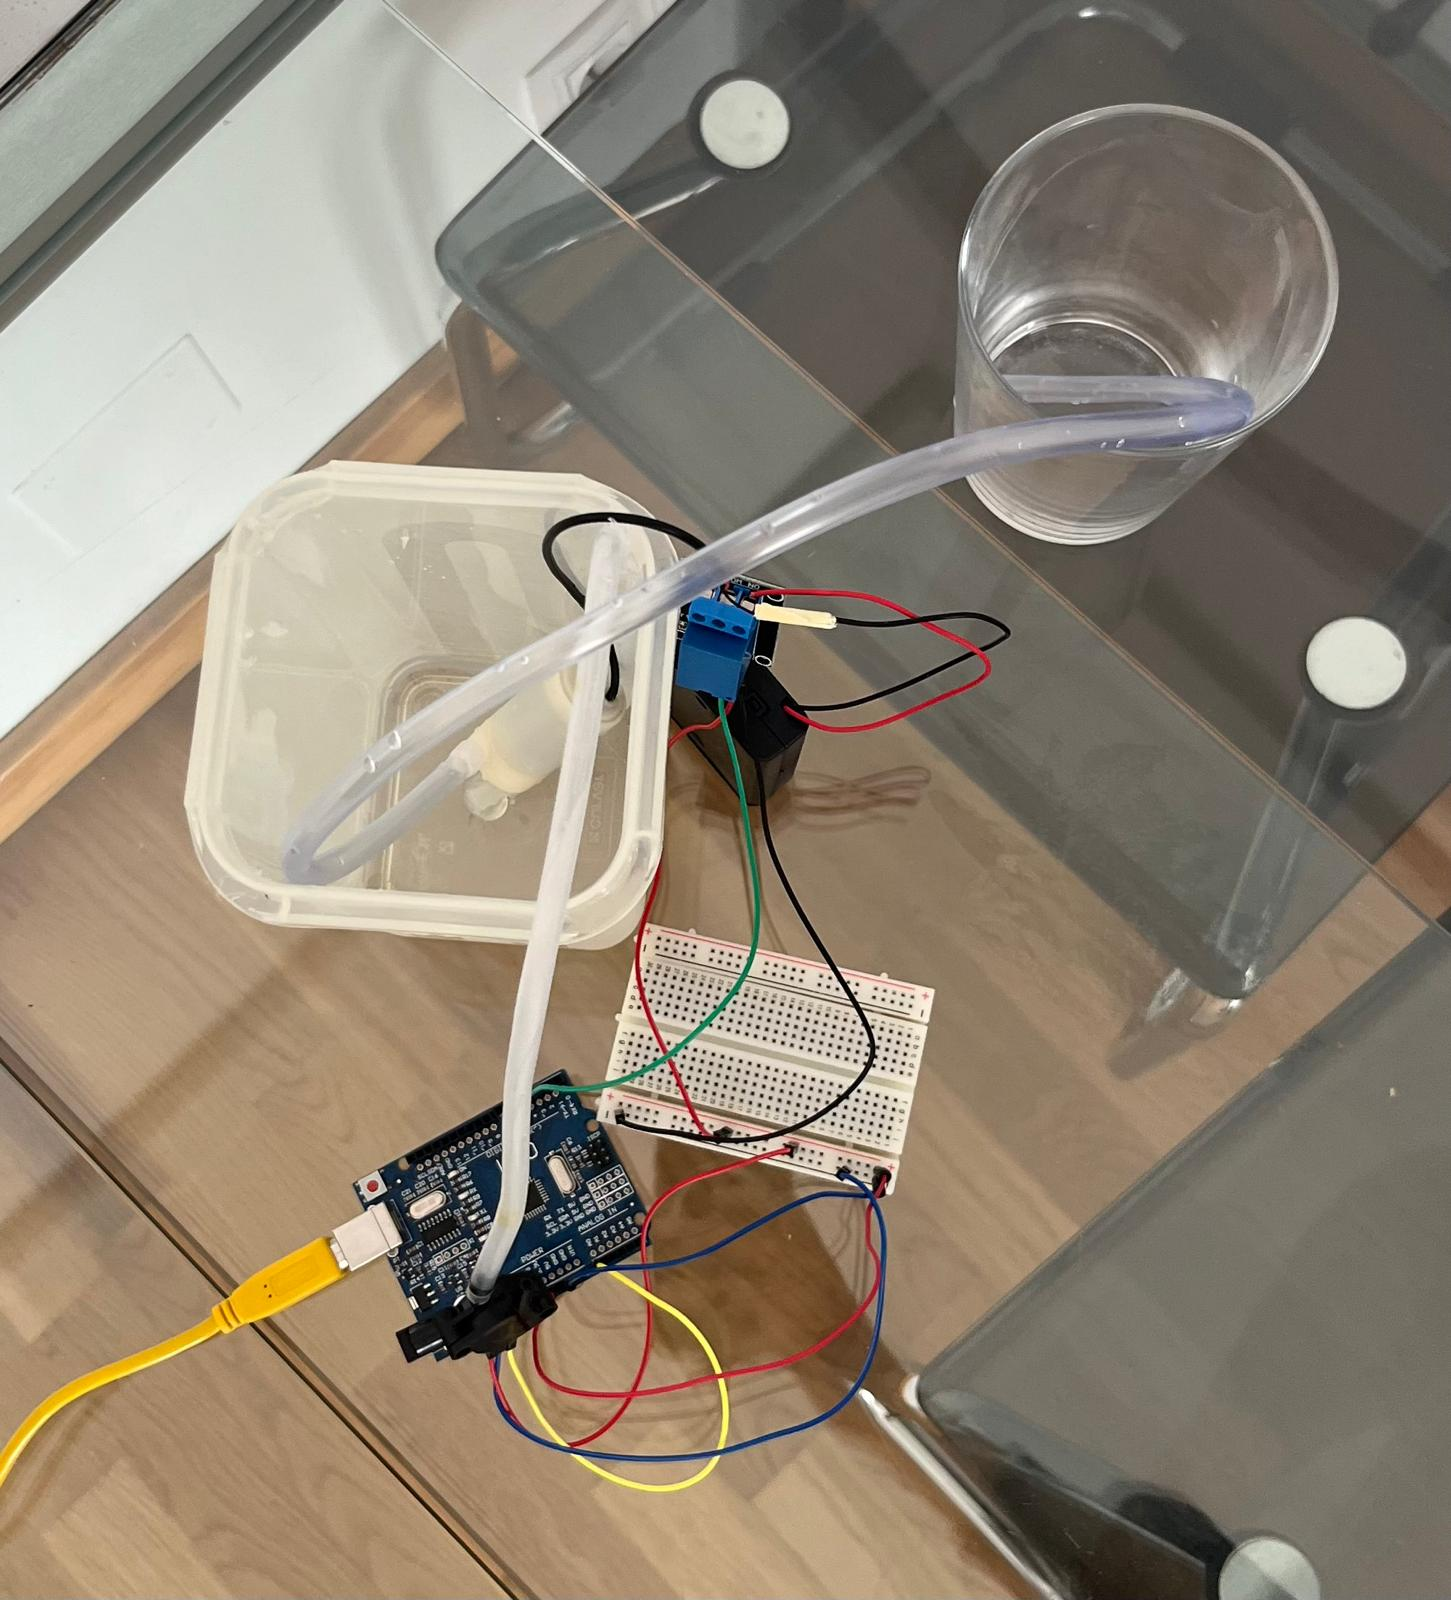
\includegraphics[width=0.8\textwidth]{img/conexioncontanques.jpg}
    \caption{Circuito completo con tanques. Imagen propia }
    \label{fig:completo}
\end{figure}


Una vez tengamos todo listo, haremos uso del cable USB para conectar la placa de Arduino al ordenador y ejecutar el programa. Podemos ver el código desarrollado en el Repositorio, en la carpeta Arduino encontraremos un archivo con el nombre  \textit{code-sensor.ino}, no obstante, se muestra a continuación:
\begin{lstlisting}
// Conexion de los pines del sensor y el rele
const int pinSensor = A0; // El sensor esta conectado al pin analogico A0
const int rele = 4; // El rele esta conectado al pin digital 4

// Variables para realizar las lecturas del sensor
double Vs = 5.0; // Voltaje de alimentacion del sensor --> 5V
double Vout; //Voltaje de salida
double P;
double P1;
double P2;
double Tol = 0.48; // Ajuste para calibrar la medida del sensor

// Datos solicitados
String nombreCompleto = "";
int anoNacimiento = 0;
String usuario = "";
String contrasena = "";
bool datosCompletos = false; //Variable booleana para controlar si los datos han sido completados y asi poder empezar a realizar las lecturas


bool bombaActivada = false; //Variable booleana para controlar si la minibomba se ha activado

void setup() {
  Serial.begin(9600);

  pinMode(rele, OUTPUT); //Configuracion del rele como salida
  digitalWrite(rele, LOW); //Inicialmente el rele esta apagado
  
  Serial.println("Por favor, introduce tu nombre completo:"); // Solicita los datos al usuario
}

void loop() {
  if (!datosCompletos) {
    //Entrada de datos por pantalla
    if (Serial.available() > 0) {
      if (nombreCompleto == "") {
        nombreCompleto= Serial.readStringUntil('\n');
        Serial.print("Nombre completo: ");
        Serial.println(nombreCompleto);
        Serial.println("Introduce tu ano de nacimiento:");
      } else if (anoNacimiento == 0) {
        anoNacimiento= Serial.readStringUntil('\n').toInt();
        if (anoNacimiento > 2006) {
          Serial.println("Error: Debe ser mayor de edad. Introduce nuevamente:");
          anoNacimiento=0; //Reinicio del ano para volver a introducirlo
        } else {
          Serial.print("Ano de nacimiento: ");
          Serial.println(anoNacimiento);
          Serial.println("Introduce tu usuario (DNI sin letras):");
        }
      } else if (usuario == "") {
        usuario = Serial.readStringUntil('\n');
        if (usuario.length() != 8) { //El DNI tiene 8 cifras
          Serial.println("Error: El usuario debe contener exactamente 8 caracteres. Introduce nuevamente:");
          usuario = ""; // Reinicia el usuario para volver a introducirlo
        } else {
          Serial.print("Usuario: ");
          Serial.println(usuario);
          Serial.println("Introduce tu contrasena (exactamente 8 caracteres):");
        }
      } else if (contrasena == "") {
        contrasena = Serial.readStringUntil('\n');
        if (contrasena.length() != 8) {
          Serial.println("Error: La contrasena debe tener 8 caracteres. Introduce nuevamente:");
          contrasena = ""; // Reinicia la contrasena para volver a introducirlo
        } else {
          Serial.print("Contrasena: ");
          for (int i = 0; i < contrasena.length(); i++) { //Bucle for para contar los caracteres introducimos y ponerlos con *
            Serial.print('*');
          }
          Serial.println();
          datosCompletos = true; //Variable booleana a true cuando los datos esten completos y correctos
          Serial.println("Datos completados. El sensor comenzara a realizar las lecturas.");
        }
      }
    }
  } else if (!bombaActivada) {
    Vout = float(analogRead(pinSensor)) * 5.0 / 1023.; // Lectura del voltaje con analogRead() --> Leemos lo que hay en el pin A0 (V)
    P = (Vout - 0.04 * Vs) / (0.09 * Vs); // Calculamos la presion (Figura 4 datasheet) kPa
    P1 = P * 7.50062; // P1 es la presion en mmHg 1kPa = 7.50062mmHg 
    P2= P1 + Tol; 

   
    Serial.print("\n\nVoltaje:");
    Serial.print(Vout);
    Serial.println(" V");
    Serial.print("Presion:");
    Serial.print(P2);
    Serial.println(" mmHg");

    if (P2 > 4.0 && !bombaActivada) { //Cuando se detecten valores superiores a 4 mmHg --> abrir mini bomba
      Serial.println("Se han detectado valores altos de presion, activando mini bomba...");
      digitalWrite(rele, HIGH); //Activa el rele para encender la minibomba
      delay(3000); 
      digitalWrite(rele, LOW); //Desactiva el rele para apagar la minibomba
      Serial.println("Mini bomba desactivada.");
      bombaActivada = true; 
      Serial.println("Prueba completada.");
    }

    delay(1000);
  }
}
\end{lstlisting}


El primer paso después de conectar la placa será compilar y subir el código. A continuación, acceder al monitor y comenzar a introducir los datos solicitados. En la Figura \ref{fig:verificar} tenemos el orden de verificación, subida y acceso al monitor respectivamente.
\begin{figure}[h]
    \centering
    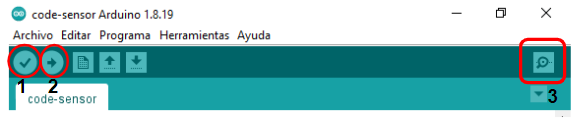
\includegraphics[width=1\textwidth]{img/compilar.PNG}
    \caption{(1) verificar, (2) subir y (3) monitor. Imagen propia }
    \label{fig:verificar}
\end{figure}


\section{Manuales y/o Demostraciones prácticas}
 Este apartado está dedicado a mostrar las demostraciones prácticas del proyecto. Una vez conectado el circuito y verificado y subido el código, procedemos a la apertura del monitor y comenzamos a completar los datos que se piden por pantalla. Primero el nombre completo (nombre y apellidos), después el año de nacimiento, usuario y por último la contraseña. En las Figuras \ref{fig:monitorINICIAL}, \ref{fig:monitorNOMBRE}, \ref{fig:monitorAÑO}, \ref{fig:monitorUSUARIO}, \ref{fig:monitorCONTRASEÑA} y \ref{fig:monitorCOMPLETO}  podemos observar este procedimiento.
 %MONITOR INICIAL
 \begin{figure}[H]
    \centering
    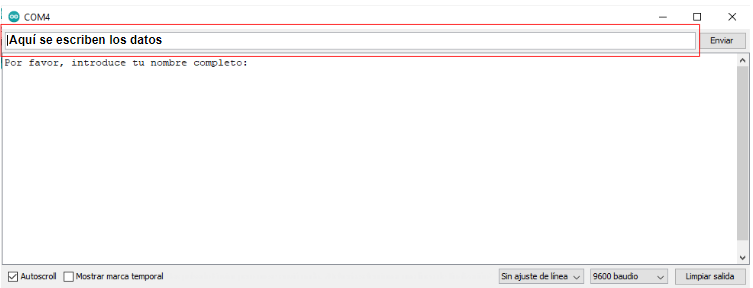
\includegraphics[width=1.3\textwidth]{img/monitorvacio.PNG}
    \caption{Estado inicial del monitor. Imagen propia }
    \label{fig:monitorINICIAL}
\end{figure}

%MONITOR NOMBRE
 \begin{figure}[H]
    \centering
    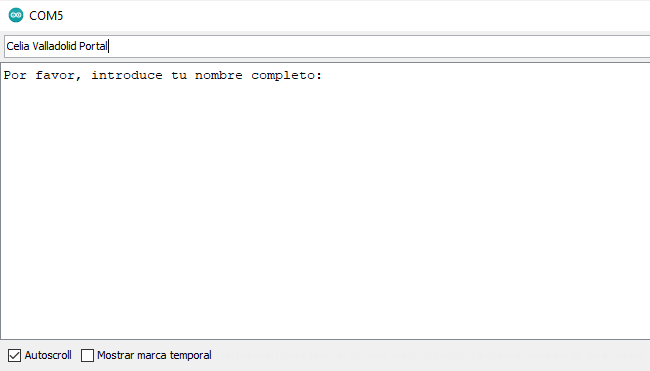
\includegraphics[width=1.1\textwidth]{img/monitornombre.PNG}
    \caption{Monitor: nombre completo. Imagen propia }
    \label{fig:monitorNOMBRE}
\end{figure}

%MONITOR AÑO
 \begin{figure}[H]
    \centering
    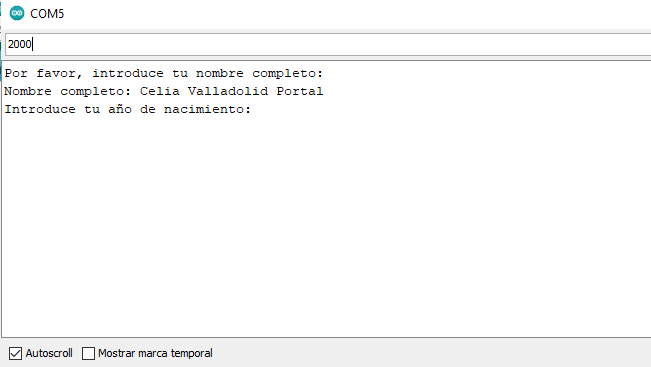
\includegraphics[width=1.1\textwidth]{img/monitoraño.PNG}
    \caption{Monitor: año de nacimiento. Imagen propia }
    \label{fig:monitorAÑO}
\end{figure}

%MONITOR USUARIO
 \begin{figure}[H]
    \centering
    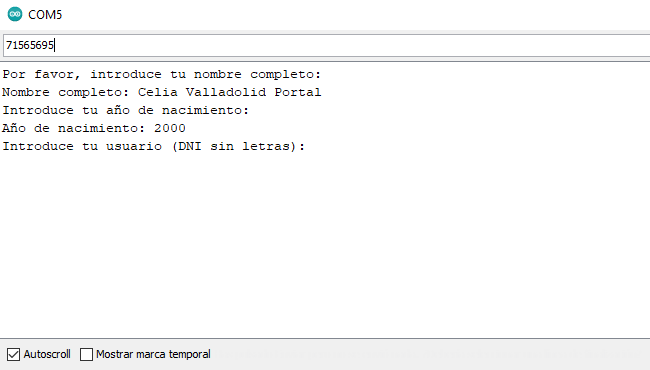
\includegraphics[width=1.1\textwidth]{img/monitorusuario.PNG}
    \caption{Monitor: usuario. Imagen propia }
    \label{fig:monitorUSUARIO}
\end{figure}

%MONITOR CONTRASEÑA
 \begin{figure}[H]
    \centering
    \includegraphics[width=1.1\textwidth]{img/monitorcontraseña.PNG}
    \caption{Monitor: contraseña. Imagen propia }
    \label{fig:monitorCONTRASEÑA}
\end{figure}

%MONITOR CON DATOS COMPLETOS
 \begin{figure}[H]
    \centering
    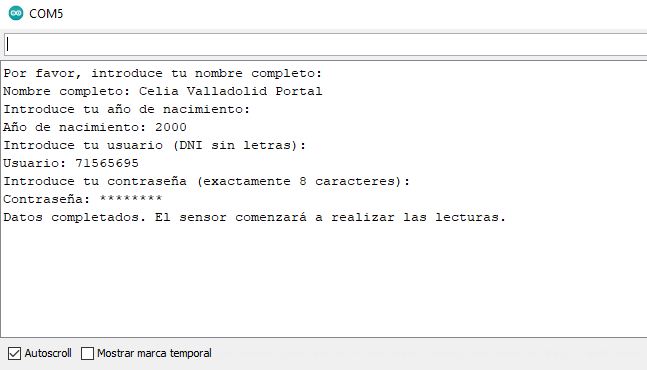
\includegraphics[width=1.1\textwidth]{img/monitorcompleto.PNG}
    \caption{Monitor con datos completos. Imagen propia }
    \label{fig:monitorCOMPLETO}
\end{figure}

Algunos campos como el año de nacimiento, el usuario y la contraseña, presentan alguna condición. Respecto al año de nacimiento, actualmente no puede ser superior a 2006, es decir, el usuario deberá de ser mayor de edad. La longitud tanto del usuario como de la contraseña será de 8 caracteres. En el caso del usuario es debido a que se corresponde con el DNI sin letra, sumando un total de 8 cifras y en el caso de la contraseña es simplemente por fijar una determinada longitud. Si alguna de estas condiciones no se cumpliera a la hora de ingresar los datos, el sistema se lo hará saber al usuario a través de un mensaje de error, ofreciéndole la oportunidad de introducir de nuevo el dato por si anteriormente hubo una confusión. Lo podemos observar en las Figuras \ref{fig:monitorAÑOMAL}, \ref{fig:monitorERRORAÑO}, \ref{fig:monitorUSUARIOMAL}, \ref{fig:monitorERRORUSUARIO}, \ref{fig:monitorCONTRASEÑAMAL}, \ref{fig:monitorERRORCONTRASEÑA} y \ref{fig:monitorFINAL} .

%MONITOR CON AÑO MAL
 \begin{figure}[h]
    \centering
    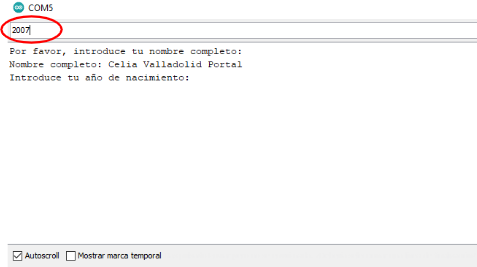
\includegraphics[width=1.1\textwidth]{img/monitorañomal.PNG}
    \caption{Monitor: introducción incorrecta del año, superior a 2006. Imagen propia }
    \label{fig:monitorAÑOMAL}
\end{figure}

%MONITOR ERROR AÑO
 \begin{figure}[h]
    \centering
    \includegraphics[width=1.1\textwidth]{img/monitorerroraño.PNG}
    \caption{Monitor: mensaje de error e introducción válida del año. Imagen propia }
    \label{fig:monitorERRORAÑO}
\end{figure}

%MONITOR CON USUARIO MAL
 \begin{figure}[h]
    \centering
    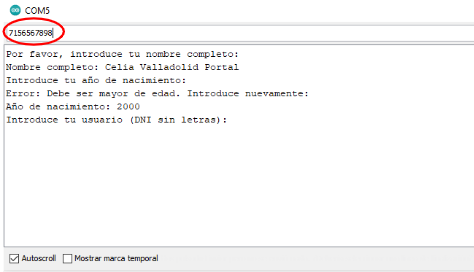
\includegraphics[width=1.1\textwidth]{img/monitorusuariomal.PNG}
    \caption{Monitor: introducción incorrecta de usuario, longitud distinta de 8. Imagen propia }
    \label{fig:monitorUSUARIOMAL}
\end{figure}

%MONITOR ERROR USUARIO
 \begin{figure}[h]
    \centering
    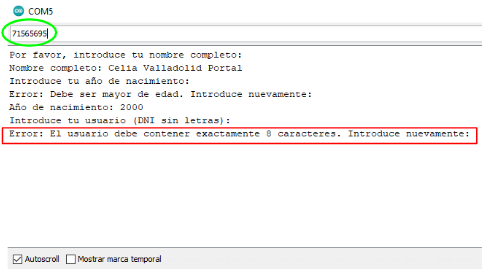
\includegraphics[width=1.1\textwidth]{img/monitorerrorusuario.PNG}
    \caption{Monitor: mensaje de error e introducción válida del usuario. Imagen propia }
    \label{fig:monitorERRORUSUARIO}
\end{figure}

%MONITOR CON CONTRASEÑA MAL
 \begin{figure}[h]
    \centering
    \includegraphics[width=1.1\textwidth]{img/monitorcontraseñamal.PNG}
    \caption{Monitor: introducción incorrecta de contraseña, longitud distinta de 8. Imagen propia }
    \label{fig:monitorCONTRASEÑAMAL}
\end{figure}

%MONITOR ERROR CONTRASEÑA
 \begin{figure}[h]
    \centering
    \includegraphics[width=1.1\textwidth]{img/monitorerrorcontraseña.PNG}
    \caption{Monitor: mensaje de error e introducción válida de contraseña. Imagen propia }
    \label{fig:monitorERRORCONTRASEÑA}
\end{figure}

%MONITOR FINAL
 \begin{figure}[h]
    \centering
    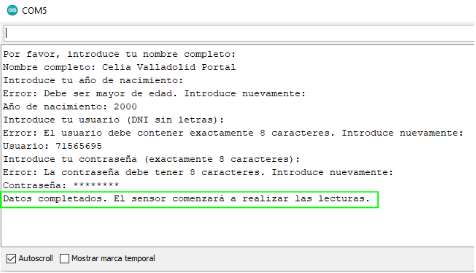
\includegraphics[width=1.1\textwidth]{img/monitorfinalbien.PNG}
    \caption{Monitor con datos completos. Imagen propia }
    \label{fig:monitorFINAL}
\end{figure}
\clearpage
Con los datos completos, el sensor comenzará a realizar lecturas de presión, detectando cambios y determinando cuando debe de activar la mini bomba para derivar el fluido de un tanque a otro.

Todas las demostraciones están contenidas en la carpeta demostraciones del Repositorio.

\apendice{Manual del programador} 

\section{Estructura de directorios}
La estructura de directorias seguida para este proyecto, está disponible en el repositorio de GitHub.

Se ha decidido optar por la siguiente estructura:
\begin{itemize} 
    \item \textbf{Carpeta img}: en esta carpeta se incluyen todas la imágenes empleadas en el proyecto, tanto para la memoria como para los anexos.
    \item \textbf{Carpeta tex}: esta carpeta está compuesta por 14 documentos LaTex (\textbf{.tex}) y 1 documento \textbf{.txt}.
    \begin{itemize}
        \item \textbf{1\_objetivos.tex}: documento que contiene la información acerca de los objetivos del proyecto, objetivo general y objetivos específicos. 
        \item \textbf{2\_abreviaturas.tex}: documento que contiene las abreviaturas y siglas empleadas en el proyecto.
        \item \textbf{3\_introduccion.tex}: documento que contiene los conceptos teóricos acerca de la hidrocefalia y estado del arte y trabajos relacionados.
        \item \textbf{4\_metodologia.tex}: documento que contiene la información relativa a los datos del proyecto y técnicas y herramientas empleadas para su desarrollo.
        \item \textbf{5\_conclusiones.tex}: documento que contiene los resultados, discusión y aspectos relevantes del proyecto.
        \item \textbf{6\_lineas\_futuras.tex}: documento que contiene información acerca de futuras mejoras del proyecto e indicaciones  e ideas sugeridas para ello.
        \item \textbf{A\_planificacion.tex}: documento que contiene la planificación del proyecto tanto temporal como económica y la viabilidad legal.
        \item \textbf{B\_manual\_usuario.tex}: documento que contiene los requisitos de software y hardware así como demostraciones del prototipo.
        \item \textbf{C\_manual\_programador.tex}: documento que contiene la estructura de directorios e instrucciones para mejoras o modificaciones futuras del proyecto.
        \item \textbf{D\_datos.tex}: documento que contiene todo lo referente a la adquisición y tratamiento de datos.
        \item \textbf{E\_diseno.tex}: documento que contiene la información referente al diseño del prototipo.
        \item \textbf{F\_requisitos.tex}: documento que contiene diagramas de casos de uso junto con su explicación.
        \item \textbf{G\_experimental.tex}: documento que contiene el cuaderno de trabajo con la explicación de los resultados tanto positivos como negativos.
        \item \textbf{H\_ODS.tex}: documento que contiene una reflexión personal acerca de los aspectos de sostenibilidad que se abordan en el proyecto.
        \item \textbf{readme.txt}: documento que contiene todas las fuentes latex para memoria y anexos.
    \end{itemize}
    \item \textbf{Carpeta memoria}: esta carpeta contiene dos archivos \textbf{.pdf} y \textbf{.tex} referentes a la memoria del proyecto.
    \begin{itemize}
        \item \textbf{memoria.pdf}: documento pdf que contiene la memoria del proyecto.
        \item \textbf{memoria.tex}: documento LaTex que contiene la estructura de la memoria del proyecto.
    \end{itemize}
    \item \textbf{Carpeta anexos}: esta carpeta contiene dos archivos \textbf{.pdf} y \textbf{.tex} referentes a los anexos del proyecto.
    \begin{itemize}
        \item \textbf{anexos.pdf}: documento pdf que contiene los anexos del proyecto.
        \item \textbf{anexos.tex}: documento LaTex que contiene la estructura de los anexos del proyecto.
    \end{itemize}
    \item \textbf{Carpeta bibliografia}: esta carpeta contiene dos archivos \textbf{.bib} referentes a la bibliografía del proyecto.
    \begin{itemize}
        \item \textbf{bibliografia.bib}: documento que contiene la bibliografía empleada en la memoria del proyecto.
        \item \textbf{bibliografiaAnexos.bib}: documento que contiene la bibliografía empleada en los anexos del proyecto.
    \end{itemize}
    \item \textbf{Carpeta arduino}: carpeta que contiene documentos \textbf{.ino} correspondientes a las pruebas realizadas y al programa completo del proyecto.
    \begin{itemize}
        \item \textbf{rele.ino}: documento que contiene el programa para probar la funcionalidad del relé.
        \item \textbf{sensor.ino}: documento que contiene el programa para probar la funcionalidad del sensor.
        \item \textbf{code-sensor.ino}: documento que contiene el programa completo del proyecto.
    \end{itemize}
    \item \textbf{Carpeta demostraciones}: carpeta que contiene tres vídeos para demostrar la funcionalidad (1) del relé, (2) del sensor y (3) del circuito completo.
    \item \textbf{datasheetMPX5010dp.pdf}: documento pdf correspondiente al datasheet del sensor empleado.
    \item \textbf{README.md}: documento de presentación del repositorio.
\end{itemize}


\section{Instrucciones para la modificación o mejora del proyecto.}

En primer lugar, sería interesante poder contar con un sensor que se pueda sumergir por completo en el agua, pudiendo realizar mediciones mucho más precisas y contar con más libertad a la hora de su manejo, evitando usar mangueras u otros utensilios para llevarlo a cabo. Estos sensores deberán contar con un encapsulado hermético para evitar la entrada de fluidos que puedan dañar el circuito.

Una mejora notable del proyecto sería la construcción de una maqueta del cráneo del paciente. Esto se podría realizar a través de una impresora 3D, simulando tanto el cráneo como el cerebro y consiguiendo generar una presión similar a la que sufre la cabeza de un paciente con hidrocefalia. De esta forma podríamos conseguir una demostración mucho más real, intentando generar presiones similares que pudiesen ser detectadas por el sensor. Debido a que en este futuro prototipo el sensor iría alojado en el interior de esta maqueta, es indispensable que fuese sumergible para su correcto funcionamiento.

Por último, el desarrollo de una aplicación. Conseguir volcar los datos generados por el sensor en un servidor en la nube que sea accesible a través de una aplicación para posteriormente poder analizarlos. Sería ideal lograr una comunicación y transmisión de datos inalámbrica, ya que si en un futuro este dispositivo ve la luz y es posible implantarlo en pacientes, es importante velar por su comodidad, estando liberados de cables que pueden limitar su libertad de movimiento.

\apendice{Descripción de adquisición y tratamiento de datos}


\section{Descripción formal de los datos}
Para la elaboración de este proyecto no se han empleado datos de fuentes externas tales como bases de datos científicas u otro tipo de fuente. Se han creado dos tipos de datos, personales y lecturas del sensor.

En cuanto a los datos personales, al inicializar el programa es necesario completar los siguientes campos para que el sensor comience a funcionar:
\begin{itemize}
    \item \textbf{Nombre completo}: variable de tipo \textit{String} que almacena el nombre completo del usuario.
    \item \textbf{Año de nacimiento}: variable de tipo \textit{int} que almacena el año de nacimiento del usuario. Debe ser mayor de edad para poder continuar.
    \item \textbf{Usuario}: variable de tipo \textit{String} que almacena el nombre de usuario. Para que sea fácil de recordar, el usuario será el DNI sin letra.
    \item \textbf{Contraseña}: variable de tipo \textit{String} que almacena la contraseña del usuario. Debe ser de una longitud de 8 caracteres y una vez ingresada se transformará en asteriscos (\textbf{*}) por temas de confidencialidad.
\end{itemize}

En total son 4 datos personales por cada usuario, nombre completo, año de nacimiento, usuario y contraseña, que serán empleados para acceder al sistema. Una vez ingresados, el sensor comenzará a realizar lecturas de los valores y cambios de presión. Ese sería el último tipo de dato generado por este programa.

En el futuro, con el desarrollo de la aplicación, se puede proceder a completar el perfil de cada usuario, incluyendo datos como el nº de historia clínica y cualquier dato que sea relevante para contar con toda la información posible del paciente.

Todos estos datos estarán debidamente protegidos en base a la legislación vigente del momento, recogida en el \textit{Anexo A, Viabilidad legal}.
\apendice{Manual de especificación de diseño}

Para este proyecto no se han realizado diagramas de clases o diagramas de despliegue.


\apendice{Especificación de Requisitos}


\section{Diagrama de casos de uso}

En la Figura \ref{fig:cu} podemos observar el diagrama de casos de uso elaborado para este proyecto. En primer lugar, se ha identificado a los actores. En este caso el único actor sería la persona encargada de desarrollar el proyecto. Después, se identifican los diferentes casos de uso. En este diagrama contamos con 7 casos de uso diferentes:

\begin{enumerate}
    \item \textbf{CU-1} Montaje del circuito electrónico. Tabla \ref{tab:cu1}
    \item \textbf{CU-2} Llenado de tanques y colocación de mangueras.Tabla \ref{tab:cu2}
    \item \textbf{CU-3} Conexión de la placa de Arduino al ordenador. Tabla \ref{tab:cu3}
    \item \textbf{CU-4} Descargar la aplicación Arduino IDE. Tabla \ref{tab:cu4}
    \item \textbf{CU-5} Ejecución del programa. Tabla \ref{tab:cu5}
    \item \textbf{CU-6} Completar los datos. Tabla \ref{tab:cu6}
    \item \textbf{CU-7} Generar datos. Tabla \ref{tab:cu7}
\end{enumerate}
\begin{figure}[h]
    \centering
    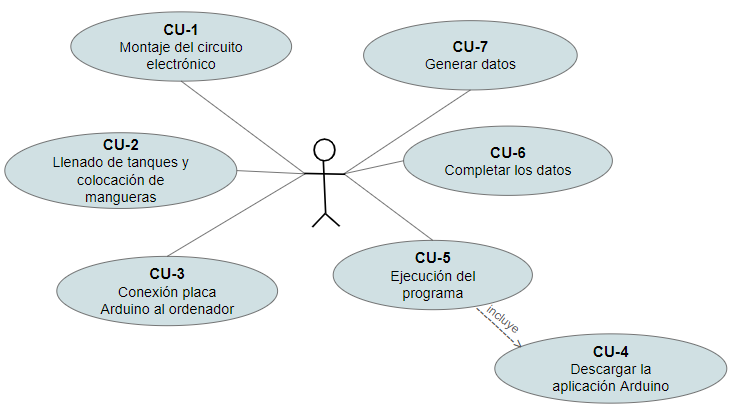
\includegraphics[width=1.2\textwidth]{img/CU.PNG}
    \caption{Diagrama de casos de uso. Imagen Propia}
    \label{fig:cu}
\end{figure}



\section{Explicación casos de uso.}

A continuación se explicarán los casos de uso mediante las tablas \ref{tab:cu1}, \ref{tab:cu2}, \ref{tab:cu3}, \ref{tab:cu4}, \ref{tab:cu5}, \ref{tab:cu6} y \ref{tab:cu7}.


% Caso de Uso 1 -> Montaje del circuito electrónico
\begin{table}[H]
	\centering
	\begin{tabularx}{\linewidth}{ p{0.21\columnwidth} p{0.71\columnwidth} }
		\toprule
            \rowcolor[HTML]{B0E0E6} 
		  \textbf{CU-1}    & \textbf{Montaje del circuito electrónico}\\
		\toprule
		\textbf{Versión}              & 1.0    \\
		\textbf{Autor}                & Celia Valladolid Portal \\
		\textbf{Descripción}          & El montaje del circuito electrónico se hará siguiendo las indicaciones recogidas en el \textit{Anexo B}. En la sección de \textit{Instalación / Puesta en marcha} podemos encontrar las instrucciones que hay que seguir para conectar todos los componentes a Arduino. \\
		\textbf{Precondición}         & Poseer todos los componentes necesarios. \\
		\textbf{Acciones}             &
		\begin{enumerate}
			\def\labelenumi{\arabic{enumi}.}
			\tightlist
                \item Conectar la placa de Arduino con la placa de pruebas.
			\item Conectar el sensor.
			\item Conectar el relé.
                \item Conectar la mini bomba y la batería.
		\end{enumerate}\\
		%\textbf{Postcondición}        & Postcondiciones (podría haber más de una) \\
		%\textbf{Excepciones}          & Excepciones \\
		\textbf{Importancia}          & Alta  \\
		\bottomrule
	\end{tabularx}
	\caption{\textbf{CU-1} Montaje del circuito electrónico.}
        \label{tab:cu1}
\end{table}

% Caso de Uso 2 -> Llenado de tanques y colocación de mangueras
\begin{table}[H]
	\centering
	\begin{tabularx}{\linewidth}{ p{0.21\columnwidth} p{0.71\columnwidth} }
		\toprule
            \rowcolor[HTML]{B0E0E6}
		\textbf{CU-2}    & \textbf{Llenado de tanques y colocación de mangueras}\\
		\toprule
		\textbf{Versión}              & 1.0    \\
		\textbf{Autor}                & Celia Valladolid Portal \\
		\textbf{Descripción}          & Colocar las mangueras en el sensor y en la mini bomba. En el caso del sensor es debido a que este no es sumergible y en el caso de la mini bomba para hacer pasar el agua. \\
		\textbf{Precondición}         & Tener montado el circuito. \\
		\textbf{Acciones}             &
		\begin{enumerate}
			\def\labelenumi{\arabic{enumi}.}
			\tightlist
                \item Colocar la manguera en uno de los puertos del sensor que haga de colchón de aire.
			\item Colocar otra manguera en la mini bomba.
                \item Llenar dos recipientes con agua, uno para el sensor y otro para la mini bomba.
		\end{enumerate}\\
		\textbf{CU relacionados}        & CU-1 \\
		%\textbf{Excepciones}          & Excepciones \\
		\textbf{Importancia}          & Alta  \\
		\bottomrule
	\end{tabularx}
	\caption{\textbf{CU-2} Llenado de tanques y colocación de mangueras.}
        \label{tab:cu2}
\end{table}

% Caso de Uso 3 -> Conexión del circuito al ordenador
\begin{table}[H]
	\centering
	\begin{tabularx}{\linewidth}{ p{0.21\columnwidth} p{0.71\columnwidth} }
		\toprule
            \rowcolor[HTML]{B0E0E6}
		\textbf{CU-3}    & \textbf{Conexión de la placa de Arduino al ordenador}\\
		\toprule
		\textbf{Versión}              & 1.0    \\
		\textbf{Autor}                & Celia Valladolid Portal \\
		\textbf{Descripción}          & Conectar la placa de Arduino al ordenador mediante el cable USB. \\
		\textbf{Precondición}         & Tener montado el circuito. \\
		\textbf{Acciones}             & Conectar el extremo USB del cable al ordenador y el otro a la placa de Arduino. \\
		\textbf{CU relacionados}        & CU-1, CU-2 \\
		%\textbf{Excepciones}          & Excepciones \\
		\textbf{Importancia}          & Alta  \\
		\bottomrule
	\end{tabularx}
	\caption{\textbf{CU-3} Conexión de la placa de Arduino al ordenador.}
        \label{tab:cu3}
\end{table}

% Caso de Uso 4 -> Descargar la app Arduino
\begin{table}[H]
	\centering
	\begin{tabularx}{\linewidth}{ p{0.21\columnwidth} p{0.71\columnwidth} }
		\toprule
            \rowcolor[HTML]{B0E0E6}
		\textbf{CU-4}    & \textbf{Descargar la aplicación Arduino IDE}\\
		\toprule
		\textbf{Versión}              & 1.0    \\
		\textbf{Autor}                & Celia Valladolid Portal \\
		\textbf{Descripción}          & Descargar la aplicación de Arduino IDE en el ordenador. Instrucciones en el \textit{Anexo B, Requisitos software}. \\
		\textbf{Precondición}         & Tener un ordenador. \\
		\textbf{Acciones}             & En el \textit{Anexo B} tenemos el enlace para descargar la aplicación. \\
		%\textbf{Excepciones}          & Excepciones \\
		\textbf{Importancia}          & Alta  \\
		\bottomrule
	\end{tabularx}
	\caption{\textbf{CU-4} Descargar la aplicación Arduino.}
        \label{tab:cu4}
\end{table}

% Caso de Uso 5 -> Cargar el programa 
\begin{table}[H]
	\centering
	\begin{tabularx}{\linewidth}{ p{0.21\columnwidth} p{0.71\columnwidth} }
		\toprule
            \rowcolor[HTML]{B0E0E6}
		\textbf{CU-5}    & \textbf{Ejecución del programa}\\
		\toprule
		\textbf{Versión}              & 1.0    \\
		\textbf{Autor}                & Celia Valladolid Portal \\
		\textbf{Descripción}          & Ejecutar el programa en la aplicación de Arduino.  \\
		\textbf{Precondición}         & Tener descargada la aplicación. \\
		\textbf{Acciones}             &
		\begin{enumerate}
			\def\labelenumi{\arabic{enumi}.}
			\tightlist
                \item Abrir la aplicación.
			\item Abrir el archivo \textit{code-sensor.ino} que podemos encontrar en la Carpeta arduino del Repositorio.
			\item Verificar y subir el código (Figura \ref{fig:verificar}).
		\end{enumerate}\\
		\textbf{CU relacionados}        & CU-1, CU-2, CU-3, CU-4 \\
		%\textbf{Excepciones}          & Excepciones \\
		\textbf{Importancia}          & Alta  \\
		\bottomrule
	\end{tabularx}
	\caption{\textbf{CU-5} Ejecución del programa.}
        \label{tab:cu5}
\end{table}

% Caso de Uso 6 -> Completar los datos
\begin{table}[H]
	\centering
	\begin{tabularx}{\linewidth}{ p{0.21\columnwidth} p{0.71\columnwidth} }
		\toprule
            \rowcolor[HTML]{B0E0E6}
		\textbf{CU-6}    & \textbf{Completar los datos}\\
		\toprule
		\textbf{Versión}              & 1.0    \\
		\textbf{Autor}                & Celia Valladolid Portal \\
		\textbf{Descripción}          & Completar los datos solicitados por el programa rellenando los campos de forma adecuada.  \\
		\textbf{Precondición}         & Haber ejecutado el programa. \\
		\textbf{Acciones}             &
		\begin{enumerate}
			\def\labelenumi{\arabic{enumi}.}
			\tightlist
                \item Abrir el monitor, paso 3 Figura \ref{fig:verificar}.
			\item Introducir nombre completo.
			\item Introducir año de nacimiento.
                \item Introducir usuario.
                \item Introducir contraseña.
		\end{enumerate}\\
		\textbf{CU relacionados}        & CU-1, CU-2, CU-3, CU-4 \\
		\textbf{Observaciones}          & Algunos campos como el año de nacimiento, usuario y contraseña, presentan restricciones. Consultar \textit{Anexo D}. \\
		\textbf{Importancia}          & Alta  \\
		\bottomrule
	\end{tabularx}
	\caption{\textbf{CU-6} Completar los datos.}
        \label{tab:cu6}
\end{table}

% Caso de Uso 7 -> Generar datos
\begin{table}[H]
	\centering
	\begin{tabularx}{\linewidth}{ p{0.21\columnwidth} p{0.71\columnwidth} }
		\toprule
            \rowcolor[HTML]{B0E0E6}
		\textbf{CU-7}    & \textbf{Generar datos}\\
		\toprule
		\textbf{Versión}              & 1.0    \\
		\textbf{Autor}                & Celia Valladolid Portal \\
		\textbf{Descripción}          & Tras haber completado correctamente los datos solicitados, el sensor empieza a realizar lecturas, identificando los cambios de presión para que la mini bomba se active al detectar un aumento dejando pasar el agua.  \\
		\textbf{Precondición}         & Haber rellenado los datos. \\
		\textbf{Acciones}             & Generar cambios de presión en el tanque donde está el sensor, para que los detecte y la mini bomba se encienda. \\
		\textbf{CU relacionados}        & CU-1, CU-2, CU-3, CU-4, CU-5 \\
		%\textbf{Excepciones}          & Excepciones \\
		\textbf{Importancia}          & Alta  \\
		\bottomrule
	\end{tabularx}
	\caption{\textbf{CU-7} Generar datos.}
        \label{tab:cu7}
\end{table}
\newpage


\section{Prototipos de interfaz o interacción con el proyecto}
Para este proyecto no se ha llegado a desarrollar una aplicación móvil que monitorice al paciente, se ha planteado como una mejora futura. No obstante, se han elaborado prototipos de la interfaz de la aplicación. En la Figura \ref{fig:inise} podemos observar la pantalla de inicio de sesión, la Figura \ref{fig:regis} se corresponde con el registro del usuario, la pantalla inicial una vez dentro de la aplicación la podemos ver en la Figura \ref{fig:appini} y por último la Figura \ref{fig:appalerta} refleja la notificación de alerta de un paciente que está sufriendo un aumento de la presión intracraneal en ese momento.

\begin{figure}[H]
    \centering
    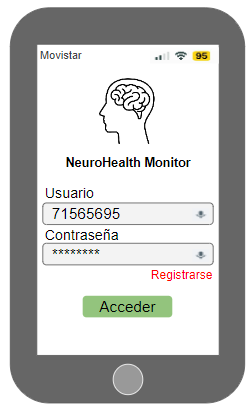
\includegraphics[width=0.4\textwidth]{img/appinicio.PNG}
    \caption{Prototipo interfaz: Inicio de sesión. Imagen propia}
    \label{fig:inise}
\end{figure}

\begin{figure}[h]
    \centering
    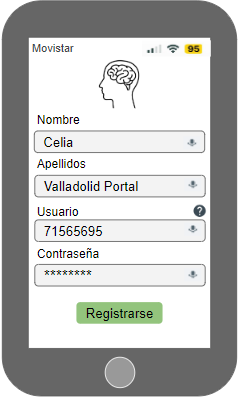
\includegraphics[width=0.4\textwidth]{img/registroapp.PNG}
    \caption{Prototipo interfaz: Registro. Imagen propia}
    \label{fig:regis}
\end{figure}

\begin{figure}[h]
    \centering
    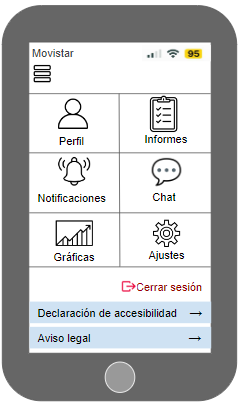
\includegraphics[width=0.4\textwidth]{img/pantallainicioapp.PNG}
    \caption{Prototipo interfaz: Pantalla inicial. Imagen propia}
    \label{fig:appini}
\end{figure}

\begin{figure}[h]
    \centering
    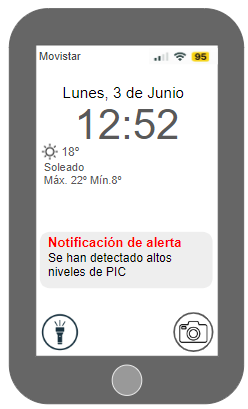
\includegraphics[width=0.4\textwidth]{img/appbloqueo.PNG}
    \caption{Prototipo interfaz: Notificación de alerta. Imagen propia}
    \label{fig:appalerta}
\end{figure}
\apendice{Estudio experimental}

Este apartado está dedicado a describir las diferentes pruebas realizadas a lo largo de la elaboración del proyecto para demostrar su funcionalidad. 

\section{Cuaderno de trabajo}

El desarrollo experimental del proyecto lo podemos dividir en dos bloques: pruebas con el relé y la mini bomba y pruebas con el sensor. Estas pruebas se han realizado para verificar que todos los componentes funcionan de forma adecuada.

\subsection{Relé}
Para probar que el relé y la mini bomba funcionan correctamente, he desarrollado un código basado en la activación del relé para encender y apagar la bomba. Para ello el primer paso es realizar las conexiones tal y como se explica en el \textit{Anexo B} en la Figura \ref{fig:conex_rele}. Una vez hecho, introduciremos la mini bomba en un recipiente con agua y conectaremos una manguera que vaya de la mini bomba a otro recipiente vacío para echar el agua. Esto lo podemos observar en la Figura \ref{fig:conex_rele_bomba}.
\begin{figure}[H]
    \centering
    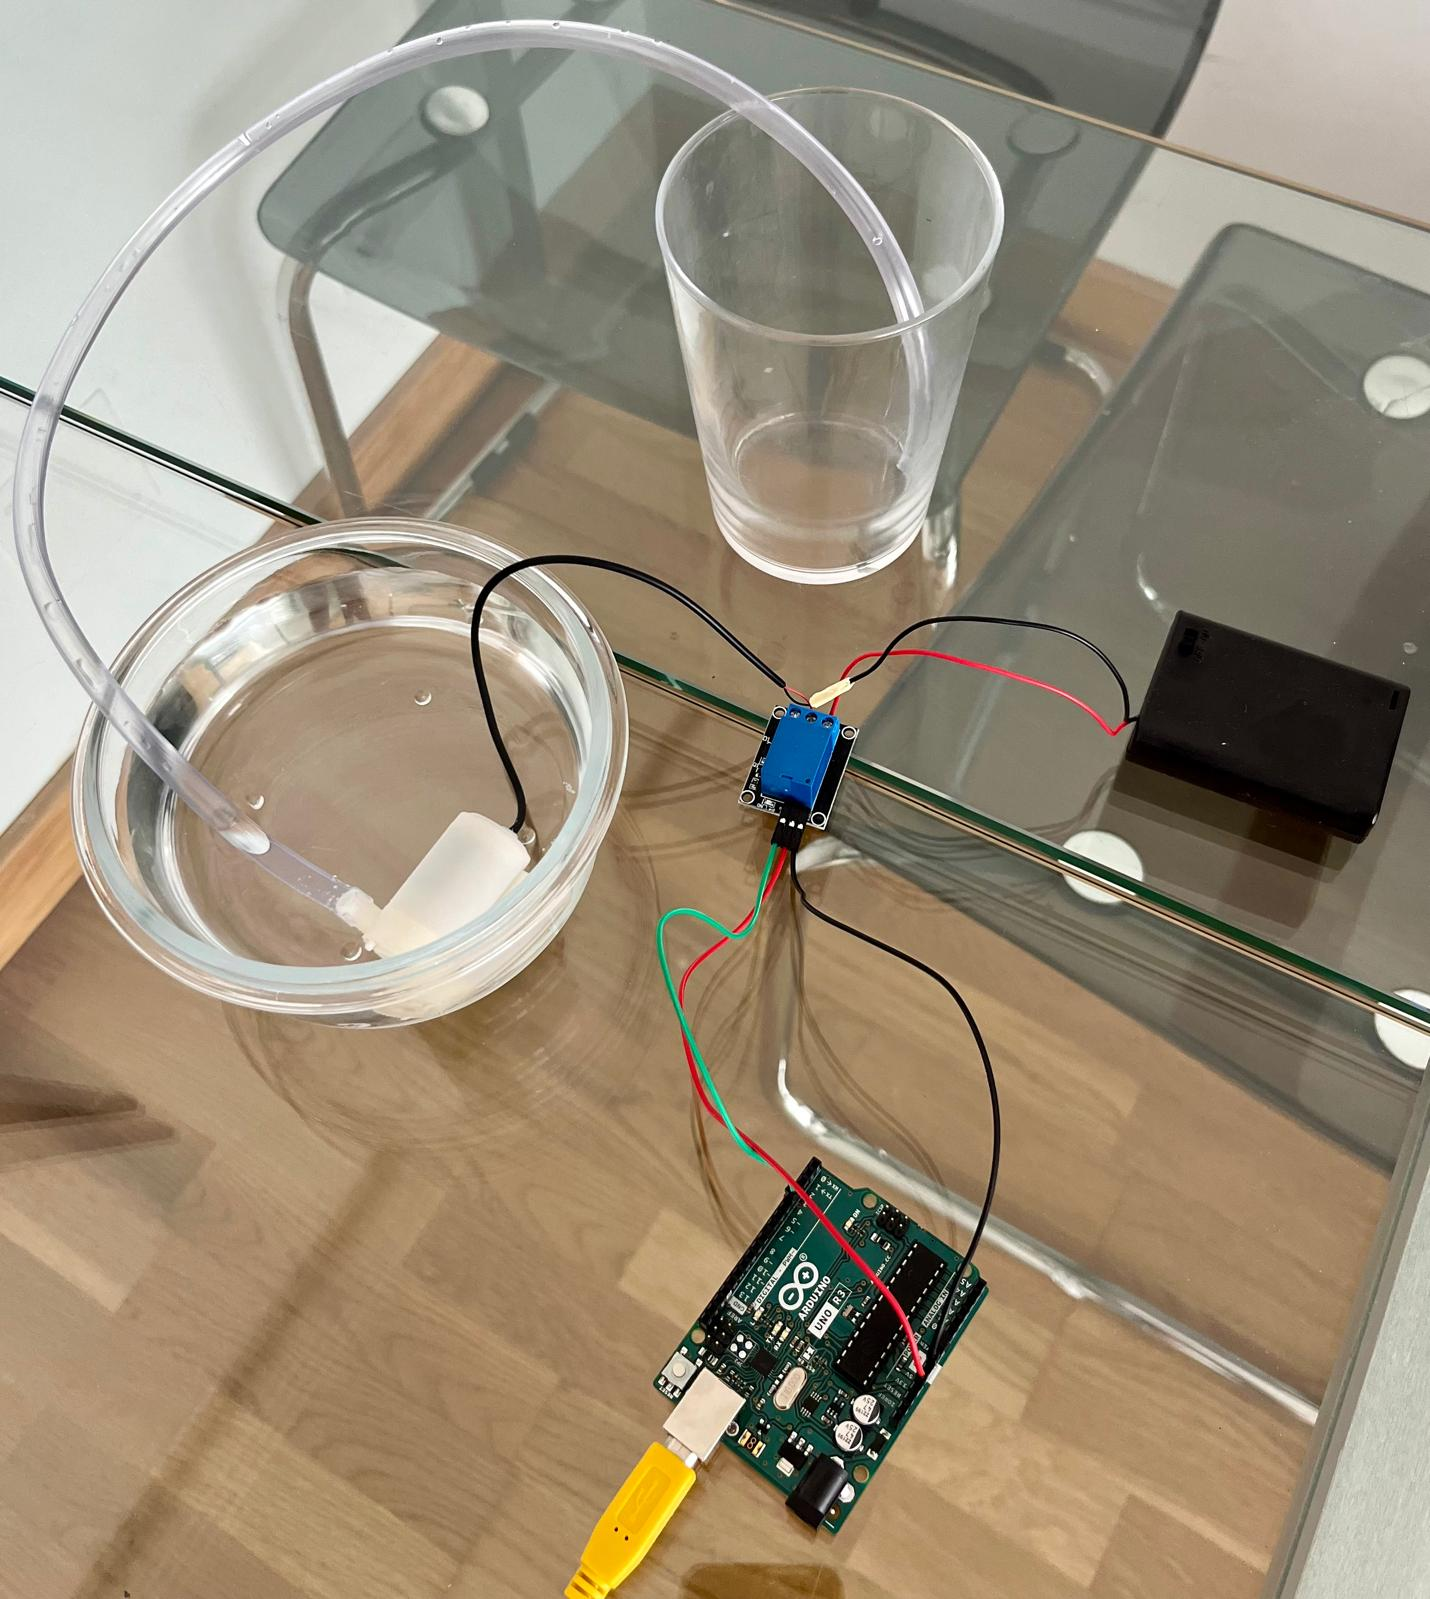
\includegraphics[width=0.7\textwidth]{img/releBomba.jpg}
    \caption{Conexión relé y mini bomba con tanques de agua. Imagen propia}
    \label{fig:conex_rele_bomba}
\end{figure}


El código desarrollado es el siguiente:

\begin{lstlisting}
const int rele = 4; // El rele esta conectado al pin digital 4
int contador = 0; // Contador para limitar el numero de veces que el rele se activa para encender la mini bomba
bool pruebaCompletada = false; // Variable booleana inicializada a false para controlar cuando la prueba ha finalizado

void setup() {
  Serial.begin(9600);
  pinMode(rele, OUTPUT); // Configuracion del rele como salida
  digitalWrite(rele, LOW); // Inicialmente el rele esta apagado
}

void loop() {
  if (!pruebaCompletada && contador < 2) { 

    // ACTIVAR MINI BOMBA
    Serial.println("Activando la mini bomba...");
    digitalWrite(rele, HIGH); // Activa el rele para encender la bomba durante 1,5 seg
    delay(1500); 
    
    // DESACTIVAR MINI BOMBA
    Serial.println("Bomba desactivada");
    digitalWrite(rele, LOW); // Desactiva el rele para apagar la bomba
    delay(3000);
    
    contador++;
     
  } else if (!pruebaCompletada) {
    Serial.println("Prueba completada"); 
    pruebaCompletada = true; // La prueba ha sido completada
    delay(1000); 
    return; 
  }
}
\end{lstlisting}

En el Repositorio, dentro de la carpeta Arduino, podemos encontrar el documento \textit{rele.ino}, que contiene el código anterior, mientras que en la carpeta demostraciones podemos encontrar un vídeo \textit{rele.mp4} demostrando que funciona correctamente.

\subsection{Sensor de presión NPX MPX5010DP}
Al igual que con el relé, se han realizado pruebas con el sensor para demostrar su funcionalidad. Para ello necesitamos realizar las conexiones de forma adecuada, tal y como indica la Figura \ref{fig:conex_sens} y poner la manguera en el sensor para crear un colchón de aire, ya que como hemos mencionado en apartados anteriores, este sensor no es sumergible. Esta manguera la hemos pegado con silicona a un recipiente, al cual iremos añadiendo agua para aumentar la presión. Lo podemos observar en la Figura \ref{fig:conex_sen_tanq}.
\begin{figure}[h]
    \centering
    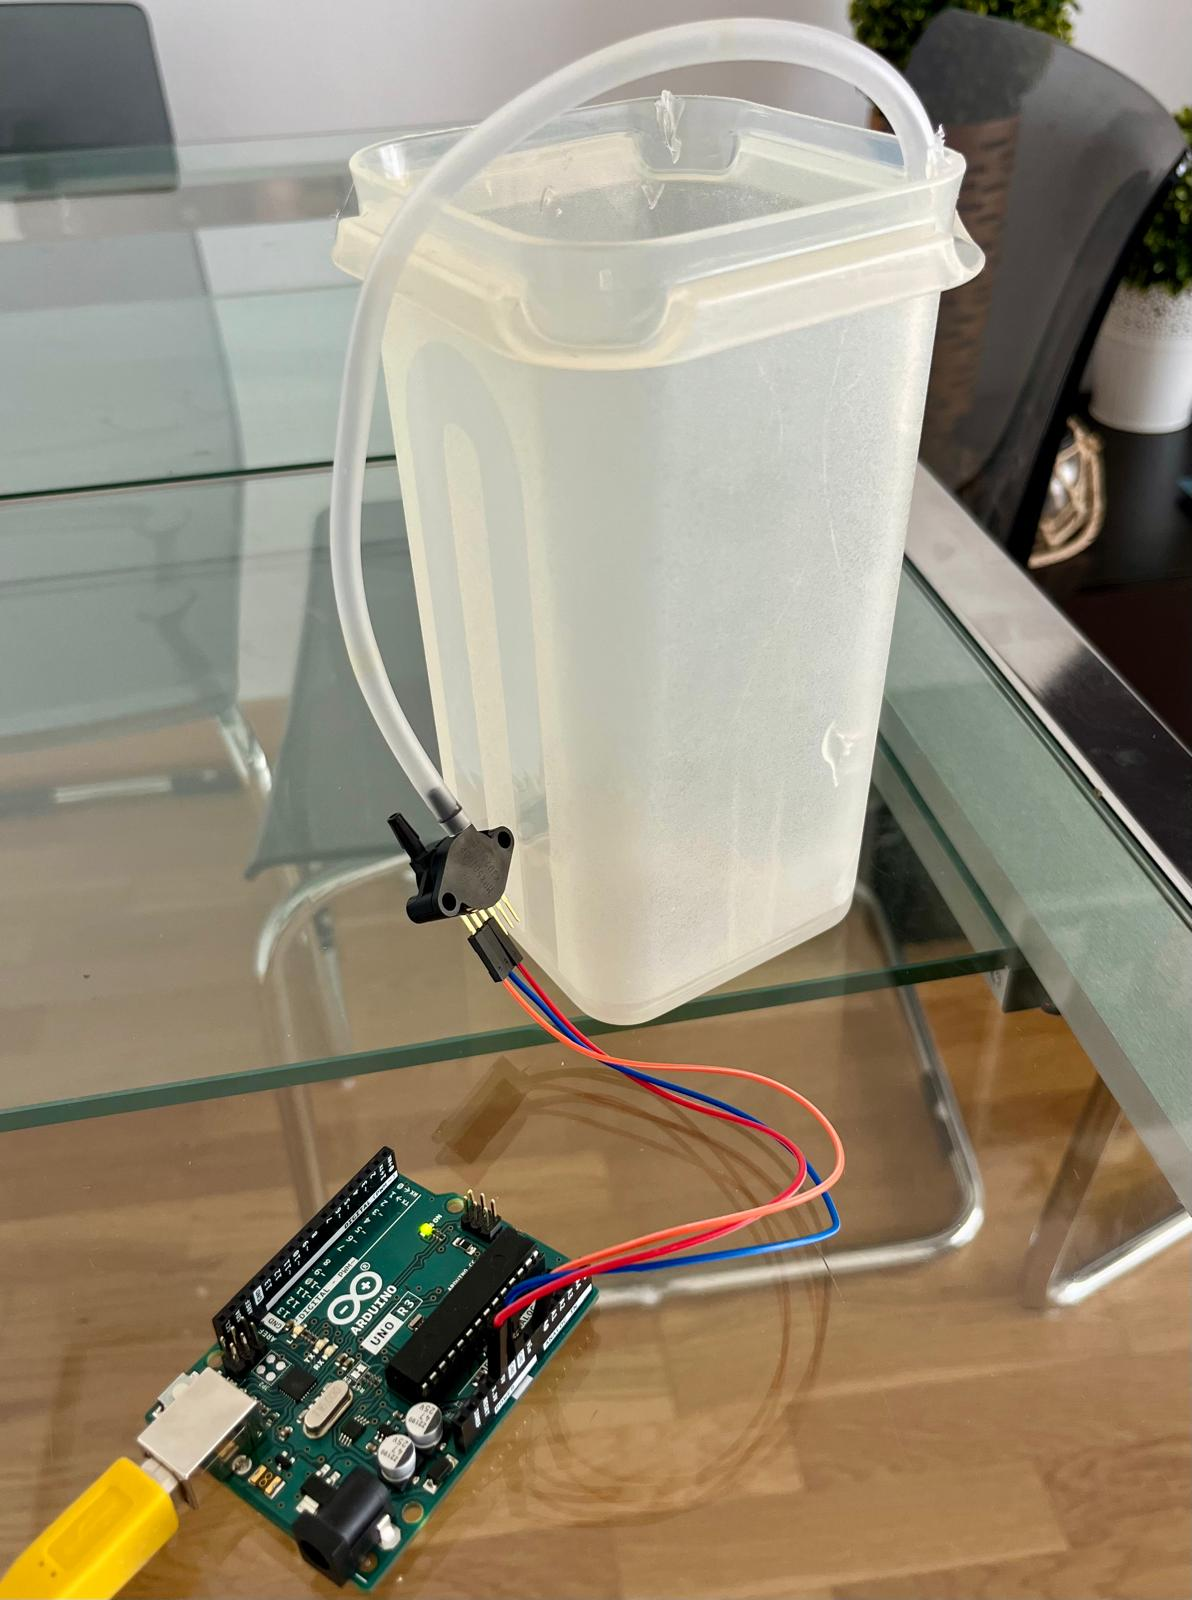
\includegraphics[width=0.6\textwidth]{img/sensortanque.jpg}
    \caption{Conexión del sensor con tanque de agua. Imagen propia}
    \label{fig:conex_sen_tanq}
\end{figure}

Cuando conectamos la placa de Arduino al ordenador y compilamos el programa, el sensor hace lecturas negativas de -0.56 mmHg \footnote{Este valor no siempre es ese, puede variar y hay que calibrarlo al inicio de cada uso.}, cuando debería de dar 0.00 mmHg ya que el recipiente está vacío. Para solucionarlo basta con sumar +0.56 al valor final de presión, para que así las lecturas con el tanque vacío sean de 0.00 mmHg. Lo podemos observar en las Figuras \ref{fig:lect-neg}, \ref{fig:tol} y \ref{fig:lectcero}.
\begin{figure}[H]
    \centering
    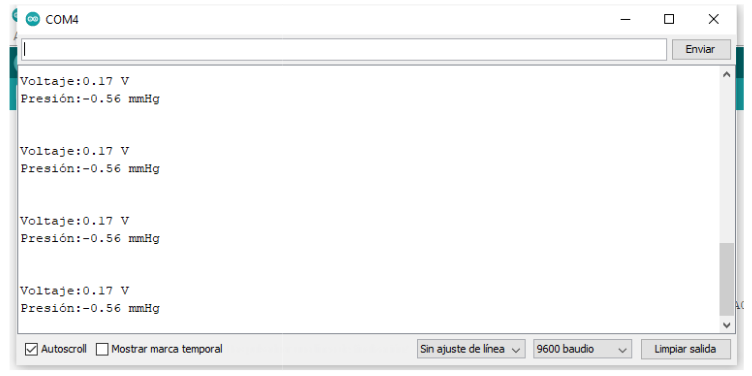
\includegraphics[width=1\textwidth]{img/lecturasnegativas.PNG}
    \caption{Lecturas negativas del sensor. Imagen propia}
    \label{fig:lect-neg}
\end{figure}

\begin{figure}[H]
    \centering
    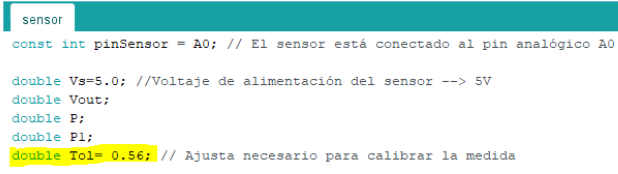
\includegraphics[width=1\textwidth]{img/tol.PNG}
    \caption{Tolerancia. Imagen propia}
    \label{fig:tol}
\end{figure}

\begin{figure}[H]
    \centering
    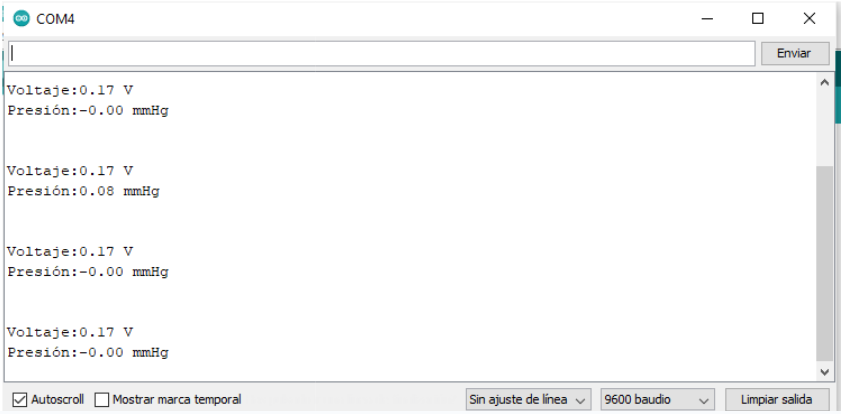
\includegraphics[width=1\textwidth]{img/lectcero.PNG}
    \caption{Sensor calibrado, lecturas iniciales correctas. Imagen propia}
    \label{fig:lectcero}
\end{figure}

Una vez calibrado, comenzamos a echar agua para que la presión aumente. Esto lo podemos ver en el vídeo \textit{sensor.mp4} contenido en la carpeta demostraciones del Repositorio. También podemos encontrar el documento \textit{sensor.ino}, que contiene el siguiente código.

\begin{lstlisting}
const int pinSensor = A0; // El sensor esta conectado al pin analogico A0

double Vs=5.0; //Voltaje de alimentacion del sensor --> 5V
double Vout;
double P; 
double P1;
double Tol= 0.56; // Ajusta necesario para calibrar la medida


void setup()
{
  Serial.begin(9600);
  
}
void loop() {
    
    Vout = float(analogRead(pinSensor))*5.0/1023.; //Lectura del voltaje con analogRead() --> Leemos lo que hay en el pin A0 (V)
  
    P = (Vout-0.04*Vs) / (0.09*Vs); //Calculamos la presion (Figura 4 datasheet)kPa
    P1 = P*7.50062+Tol; //P1 es la presion en mmHg 1kPa = 7.50062mmHg 
    
    Serial.print("\n\nVoltaje:");
    Serial.print(Vout);
    Serial.println(" V");
    Serial.print("Presion:");
    Serial.print(P1);
    Serial.println(" mmHg");
  
    delay(5000);
    
  }
\end{lstlisting}

\section{Observaciones}
En este proyecto se ha empleado la presión hidrostática\footnote{La presión hidrostática es la presión a la que está sometido un cuerpo sumergido en un fluido, debido a la columna de líquido que tiene sobre él \cite{presionhidro}.} del agua, cuya fórmula es la siguiente: 
\[
P = \rho g h
\]

donde:
\begin{itemize}
    \item \( P \): presión hidrostática,
    \item \( \rho \): densidad del agua,
    \item \( g \): fuerza de gravedad,
    \item \( h \): altura de la columna de agua.
\end{itemize}

La presión ha ido aumentando a medida que se echaba más agua al tanque, es decir, con la altura, ya que la gravedad y la densidad del agua han permanecido constantes en todo momento.
\apendice{Anexo de sostenibilización curricular}

\section{Reflexión personal sobre los aspectos de sostenibilidad}

El desarrollo de tecnologías médicas debe tener en cuenta la sostenibilidad, y este Trabajo de Fin de Grado centrado en el desarrollo de una válvula de derivación ventriculoperitoneal que integra un sensor para medir los valores de presión intracraneal y controlar la apertura de la válvula en función de las lecturas que realice, aborda numerosos aspectos relacionados con la sostenibilidad y los derechos fundamentales. A continuación, se examinarán estos elementos y las habilidades adquiridas durante la elaboración del presente proyecto, en relación con las disposiciones del \textbf{Real Decreto 822/2021} \cite{anexoH-realdecre}.

\subsection{Derechos humanos y derechos fundamentales}
El proyecto demuestra un respeto profundo por los \textbf{derechos humanos}\footnote{Los derechos humanos, recogidos en la Declaración Universal de los Derechos Humanos (DUDH), son los derechos que tiene una persona desde su nacimiento por el simple hecho de existir y se reconocen a todas las personas del mundo. Los derechos fundamentales tienen un alcance nacional, y dependiendo del país, pueden cambiar.} \cite{dere-hum} y los \textbf{derechos fundamentales} \cite{dere-funda}, que son fundamentales para el avance tecnológico, especialmente en el ámbito médico. El objetivo del prototipo desarrollado en este trabajo es mejorar significativamente la calidad de vida de los pacientes con hidrocefalia, ofreciendo un método efectivo, preciso y automatizado para controlar la presión intracraneal del paciente. Este método fomenta los valores democráticos y la equidad al garantizar que todos los pacientes, independientemente de su origen o condición, puedan beneficiarse de las innovaciones médicas, respetando su dignidad y sus derechos.
    
\subsection{Igualdad de género y no discriminación}
En el desarrollo de este proyecto, se ha adoptado una perspectiva inclusiva que respeta la igualdad de género y la no discriminación. La \textbf{Ley Orgánica 3/2007, de 22 de marzo, para la igualdad efectiva de mujeres y hombres} \cite{ley-igualdad} subraya la importancia de eliminar cualquier forma de discriminación. En este sentido, el proyecto ha asegurado que tanto el desarrollo como el posterior uso de la válvula sean accesibles para todos los pacientes, sin importar su género, edad, origen étnico, o cualquier otra condición. Además, si en un futuro se retoma el proyecto incluyendo las mejoras citadas en apartados anteriores, la composición del equipo de desarrollo y las oportunidades de participación serán equitativas, fomentando y promoviendo un entorno de trabajo inclusivo y diverso.

\subsection{Accesibilidad universal y diseño para todas las personas}
El respeto a los principios de accesibilidad universal y diseño para todas las personas es otro componente a tener en cuenta en este proyecto. Esta válvula ha sido diseñada teniendo en cuenta las necesidades de personas que padecen hidrocefalia, incluidos aquellos con discapacidades. La futura aplicación para poder monitorizar al paciente contará con una interfaz sencilla, siendo fácil de usar y estando adaptada a los requerimientos de los pacientes. Este enfoque asegura que el dispositivo junto con la aplicación no solo sean efectivos en su función principal sino que también sean accesibles para cualquier persona que lo necesite, promoviendo una mayor inclusión en la atención médica.

\subsection{Sostenibilidad y cambio climático}
El tratamiento de la sostenibilidad y del cambio climático es una potente consideración hoy en día, de acuerdo con la \textbf{Ley 7/2021, de 20 de mayo, de cambio climático y transición energética} \cite{ley-cc}. La selección de materiales y la metodología de desarrollo deben ir orientados a minimizar el impacto ambiental, empleando componentes eficientes y duraderos para evitar ser reemplazados a corto plazo. Estos serían algunos aspectos a tener en cuenta:
\begin{enumerate}
    \item \textbf{Selección de materiales sostenibles}: optar por materiales reciclables, biodegradables o que necesiten menos energía para su fabricación.
    \item \textbf{Eficiencia energética}: enfocar el diseño de los dispositivos hacia la reducción del consumo de energía, empleando fuentes de energía renovable.
    \item \textbf{Durabilidad}: crear dispositivos duraderos, con componentes resistentes que no necesiten ser cambiados de forma frecuente.
    \item \textbf{Reducción de residuos}: fomentar el reciclaje y la reutilización de componentes, diseñando productos modulares para que en el caso de tener que repararlos no se generen tantos residuos ya que se podrá cambiar únicamente el componente dañado.
    \item \textbf{Compromiso e investigación}: mantener un compromiso con la sostenibilidad y la disminución del impacto climático invirtiendo en investigación para desarrollar nuevas tecnologías a través de prácticas más respetuosas con el medio ambiente.
\end{enumerate}

A lo largo del desarrollo de este proyecto se han adquirido y aplicado diferentes competencias acerca de la sostenibilidad. Entre ellas destacan la capacidad para desarrollar un producto accesible para todo el mundo independientemente del género, edad, origen étnico o presencia de alguna discapacidad promoviendo la igualdad y la no discriminación, y la adquisición de conocimiento referente a las leyes vigentes que tratan del cambio climático y promueven la sosteniblidad. Este proyecto sirve para sentar las bases que se deben seguir en un futuro para desarrollar dispositivos médicos tecnológicos que sean duraderos, eficientes y respetuosos con el medio ambiente.



%\bibliographystyle{apalike}
\bibliographystyle{unsrt}
\bibliography{bibliografia/bibliografiaAnexos}

\end{document}
